\section{Identical Particles}
\subsection*{Sol. 1}
\begin{enumerate}
    \item 
    \begin{align*}
        \bm R + \frac{\mu}{m_1}\bm r= 
        \frac{m_1\bm r_1+m_2\bm r_2}{m_1+m_2}
        +
        \frac{m_2}{m_1+m_2}
        (\bm r_1-\bm r_2)
        =\bm r_1
    \end{align*}
    \begin{align*}
        \bm R - \frac{\mu}{m_1}\bm r= 
        \frac{m_1\bm r_1+m_2\bm r_2}{m_1+m_2}
        -
        \frac{m_2}{m_1+m_2}
        (\bm r_1-\bm r_2)
        =\bm r_2
    \end{align*}
    By the chain rule
    \begin{align*}
        \begin{pmatrix}
        \nabla_R(g\circ f) && \nabla_r(g\circ f)
        \end{pmatrix}
        =&
        \begin{pmatrix}
        \nabla_1 g && \nabla_2g
        \end{pmatrix}
        \begin{pmatrix}
            \frac{\partial f_1}{\partial R} & \frac{\partial f_1}{\partial r}\\
            \frac{\partial f_2}{\partial R} & \frac{\partial f_2}{\partial r}
        \end{pmatrix}\\
        =&
        \begin{pmatrix}
        \nabla_1 g && \nabla_2g
        \end{pmatrix}
        \begin{pmatrix}
            1 & \frac{\mu}{m_1}\\
            1 & -\frac{\mu}{m_2}
        \end{pmatrix},
    \end{align*}
    $$
    \begin{pmatrix}
            1 & \frac{\mu}{m_1}\\
            1 & -\frac{\mu}{m_2}
        \end{pmatrix}^{-1}
        =\begin{pmatrix}
            \frac{\mu}{m_2} & \frac{\mu}{m_1}\\
            1 & -1
        \end{pmatrix}
    $$
    so 
    $$
    \nabla_1 = \frac{\mu}{m_2}\nabla_R +\nabla_r
    $$
    $$
    \nabla_2 = \frac{\mu}{m_1}\nabla_R -\nabla_r.
    $$
    \item 

    \begin{align*}
        -\frac{\hbar^2}{2m_1}
        (\frac{\mu}{m_2}\nabla_R +\nabla_r)^2\psi
        -\frac{\hbar^2}{2m_2}
        (\frac{\mu}{m_1}\nabla_R -\nabla_r)^2\psi
        +V(r)\psi = E\psi
    \end{align*}
    \begin{align*}
        (-\frac{\hbar^2\mu^2}{2m_1m_2^2}
        -\frac{\hbar^2\mu^2}{2m_2m_1^2})
        \nabla^2_R
        \psi 
        +
        (-\frac{\hbar^2}{2m_1}
        -\frac{\hbar^2}{2m_2})
        \nabla_r^2 \psi 
        +V(r)\psi = E\psi.
    \end{align*}
    \begin{align*}
        -\frac{\hbar^2}{2(m_1+m_2)}
        \nabla^2_R\psi 
        -
        \frac{\hbar^2}{2\mu}
        \nabla_r^2\psi + V(r)\psi = E\psi.
    \end{align*}
    \item 
    $$
    -\frac{\hbar^2}{2(m_1+m_2)}
        \nabla^2_R\psi_R(R) = E_R\psi_R(R)
    $$
    $$
    -\frac{\hbar^2}{2\mu}
        \nabla_r^2\psi_r(r) + V(r)\psi_r(r) = E_r\psi_r(r).
    $$
\end{enumerate}

\subsection*{Sol. 2}
\begin{enumerate}
    \item 
    $m_e=9.1093837\times 10^{-31}kg,$
$\mu = \frac{9.1093837\times 10^{-31}\times 1.67262192\times 10^{-27}}
{9.1093837\times 10^{-31}+1.67262192\times 10^{-27}}
\approx 9.10442527501427\times 10^{-31}kg
$

$$
\frac{E}{E_1}-1 = 
\frac{\mu}{m_e} - 1
\approx -0.05\%
$$
\item 
The modified Rydberg constant is 
$1.0964\times10^7m^{-1},$ 
$$
\frac{1}{\lambda}=
1.0964\times10^7\times(\frac{1}{4}-\frac{1}{9})
\Rightarrow \lambda\approx 6.5669\times 10^{-7}m
$$

For the deuterium, $\mu\approx 9.1069\times10^{-31}kg,$ so the 
modified Rydberg constant is  $1.0967\times10^7m^{-1},$
$$
\frac{1}{\lambda}=
1.0967\times10^7\times(\frac{1}{4}-\frac{1}{9})
\Rightarrow \lambda\approx 6.56514\times 10^{-7}m
$$

\item 
The reduced mass is only half the electron mass, so 
the binding energy for the positronium is $-6.8eV.$
\item The reduced mass is now $1.6929\times 10^{-28}kg,$ so 
the Rydberg constant is $2038689171,$ thus 
$$
\frac{1}{\lambda} = 2038689171(1-\frac{1}{4})
\Rightarrow \lambda =  6.54\times 10^{-10}m
$$


\end{enumerate}


\subsection*{Sol. 3}
The ratio of the energies for the two isotopes is 
$$
\frac{\omega_1}{\omega_2}
=\sqrt{\frac{\mu_2}{\mu_1}}
=\sqrt{\frac{m_{37}}{m_{35}}\frac{m_H+m_{35}}{m_H+m_{37}}}
=\sqrt{\frac{17+20}{17+18}\frac{17+18+1}{17+20+1}}
=1.000751,
$$
so the difference between two vibrational spectrum is 
$7.51\times 10^{-4}\nu.$

\subsection*{Sol. 4}
\begin{enumerate}
    \item 
    \begin{align*}
        &\int A^2
        (\psi_a(\bm r_1)\psi_b(\bm r_2)
        +\psi_a(\bm r_2)\psi_b(\bm r_1))^2
        d^3\bm r_1
        d^3\bm r_2\\
        =&
        A^2\int
        \psi_a(\bm r_1)^2
        \psi_b(\bm r_2)^2
        d^3\bm r_1
        d^3\bm r_2
        +
        A^2\int
        \psi_a(\bm r_2)^2
        \psi_b(\bm r_1)^2
        d^3\bm r_1
        d^3\bm r_2\\
        &+
        2A^2\int
        \psi_a(\bm r_1)
        \psi_b(\bm r_2)
        \psi_a(\bm r_2)
        \psi_b(\bm r_1)
        d^3\bm r_1
        d^3\bm r_2\\
        =&
        A^2+A^2\Rightarrow A=\frac{1}{\sqrt{2}}.
    \end{align*}
    \item 
    \begin{align*}
        &\int 4A^2
        \psi_a^2(\bm r_1)
        \psi_a^2(\bm r_2)
        d^3\bm r_1
        d^3\bm r_2
        \Rightarrow A=\frac{1}{2}.
    \end{align*}
\end{enumerate}

\subsection*{Sol. 5}
\begin{enumerate}
    \item 
    $$
    H = -\frac{\hbar^2}{2m_1}\nabla_1^2
    -\frac{\hbar^2}{2m_2}\nabla_2^2
    +V(x_1)+V(x_2),
    $$
    where $V(x)=0$ if $0<x<a,$ and $\infty$ otherwise.

    \begin{align*}
        &(-\frac{\hbar^2}{2m}\nabla_1^2
    -\frac{\hbar^2}{2m}\nabla_2^2)
        \left[
        \sin(\frac{\pi x_1}{a})
        \sin(\frac{2\pi x_2}{a})
        -
        \sin(\frac{2\pi x_1}{a})
        \sin(\frac{\pi x_2}{a})
        \right]\\
        =&
        \frac{\hbar^2}{2m}
        \frac{\pi^2}{a^2}\sin(\frac{\pi x_1}{a})
        \sin(\frac{2\pi x_2}{a})
        -
        \frac{\hbar^2}{2m}
        \frac{4\pi^2}{a^2}
        \sin(\frac{2\pi x_1}{a})
        \sin(\frac{\pi x_2}{a})\\
        &+\frac{\hbar^2}{2m}
        \frac{4\pi^2}{a^2}\sin(\frac{\pi x_1}{a})
        \sin(\frac{2\pi x_2}{a})
        -\frac{\hbar^2}{2m}
        \frac{\pi^2}{a^2}
        \sin(\frac{2\pi x_1}{a})
        \sin(\frac{\pi x_2}{a})\\
        =&
        \frac{5\hbar^2\pi^2}{2ma^2}
        \left[
        \sin(\frac{\pi x_1}{a})
        \sin(\frac{2\pi x_2}{a})
        -
        \sin(\frac{2\pi x_1}{a})
        \sin(\frac{\pi x_2}{a})
        \right]
    \end{align*}
    \item 
    The second excited state for the distinguishable particles is nondegenerate
    $$
    \psi_{22}=
    \frac{2}{a}\sin(\frac{2\pi x_1}{a})
    \sin(\frac{2\pi x_2}{a}),\; 
    E_{22}=8K,
    $$
    and the third excited state is doubly degenerate
    $$
    \psi_{13}=
    \frac{2}{a}\sin(\frac{\pi x_1}{a})
    \sin(\frac{3\pi x_2}{a}),\; 
    E_{13}=10K
    $$
    $$
    \psi_{31}=
    \frac{2}{a}\sin(\frac{3\pi x_1}{a})
    \sin(\frac{1\pi x_2}{a}).\; 
    E_{31}=10K.
    $$
    
    The second excited state for bosons is just like the distinguishable particles. The third excited state is 
    $$
    \frac{\sqrt{2}}{a}
    \left[
    \sin(\frac{\pi x_1}{a})
    \sin(\frac{3\pi x_2}{a})+
    \sin(\frac{3\pi x_1}{a})
    \sin(\frac{\pi x_2}{a})
    \right], \; 
    E = 10K.
    $$
    
    The first and second excited states for fermions are 
    $$
    \frac{\sqrt{2}}{a}
    \left[
    \sin(\frac{\pi x_1}{a})
    \sin(\frac{3\pi x_2}{a})-
    \sin(\frac{3\pi x_1}{a})
    \sin(\frac{\pi x_2}{a})
    \right],\;
    E = 10K
    $$
    and
    $$
    \frac{\sqrt{2}}{a}
    \left[
    \sin(\frac{2\pi x_1}{a})
    \sin(\frac{3\pi x_2}{a})-
    \sin(\frac{3\pi x_1}{a})
    \sin(\frac{2\pi x_2}{a})
    \right]
    , \; 
    E = 13K.
    $$
\end{enumerate}
\subsection*{Sol. 6}
Distinguishable:
   \begin{align*}
        \langle x^2\rangle_n
    +\langle x^2\rangle_l
    -2
    \langle x\rangle_n
    \langle x\rangle_l
    =&
    a^2\left(\frac{1}{3}-\frac{1}{2\pi^2n^2}    \right)
    +
    a^2\left(\frac{1}{3}-\frac{1}{2\pi^2l^2}    \right)
    -2\frac{a}{2}\frac{a}{2}\\
    =&
    a^2\left(\frac{1}{6}-\frac{1}{2\pi^2}
    \left(\frac{1}{n^2}+\frac{1}{l^2}\right)\right)
   \end{align*}
   \begin{align*}
       \langle x\rangle_{nl}
       =&\frac{2}{a}\int_0^ax\sin(\frac{n\pi}{a}x)\sin(\frac{l\pi}{a}x)dx\\
       =&\frac{1}{a}
       \int_0^a
       x\left[
       \cos(\frac{(n-l)\pi x}{a})
       -
       \cos(\frac{(n+l)\pi x}{a})
       \right]
       dx\\
       =&
       \frac{a}{(n-l)^2\pi^2}
       (\cos((n-l)\pi )-1)
       -\frac{a}{(n+l)^2\pi^2}
       (\cos((n+l)\pi )-1)
   \end{align*}
   If $n+l\equiv0\mod 2,$
   $$
   \langle x\rangle_{nl}=0,
   $$
    if $n+l\equiv0\mod 2,$
   $$
   \langle x\rangle_{nl}=
   \frac{-2a}{(n-l)^2\pi^2}-\frac{-2a}{(n+l)^2\pi^2}
   =\frac{-8anl}{(n+l)^2(n-l)^2\pi^2}.
   $$
   Bosons
   $$
   \langle(x_1-x_2)^2\rangle
   =a^2\left(\frac{1}{6}-\frac{1}{2\pi^2}
    \left(\frac{1}{n^2}+\frac{1}{l^2}\right)\right)
    -
    \left(\frac{8anl}{(n+l)^2(n-l)^2\pi^2}\right)^2
   $$
   Fermions
   $$
   \langle(x_1-x_2)^2\rangle
   =a^2\left(\frac{1}{6}-\frac{1}{2\pi^2}
    \left(\frac{1}{n^2}+\frac{1}{l^2}\right)\right)
    +
    \left(\frac{8anl}{(n+l)^2(n-l)^2\pi^2}\right)^2
   $$
   The last term is present only when $n,l$ have the same parity.
   
   
   \subsection*{Sol. 7}
   \begin{enumerate}
       \item 
       Distinguishable:
        $$
        \psi(x_1,x_2)=
        \left(
        \frac{m\omega}{\pi\hbar}
        \right)^{1/2}
        \sqrt{\frac{2m\omega}{\hbar}}
        x_2
        e^{-\frac{m\omega}{2\hbar}x_1^2}
        e^{-\frac{m\omega}{2\hbar}x_2^2}
        $$
    Bosons:
    $$
        \psi(x_1,x_2)=
        \frac{1}{\sqrt{2}}
        \left(
        \frac{m\omega}{\pi\hbar}
        \right)^{1/2}
        \sqrt{\frac{2m\omega}{\hbar}}
        \left[
        x_2
        e^{-\frac{m\omega}{2\hbar}x_1^2}
        e^{-\frac{m\omega}{2\hbar}x_2^2}
        +
        x_1
        e^{-\frac{m\omega}{2\hbar}x_1^2}
        e^{-\frac{m\omega}{2\hbar}x_2^2}
        \right]
        $$
    Fermions:
    $$
        \psi(x_1,x_2)=
        \frac{1}{\sqrt{2}}
        \left(
        \frac{m\omega}{\pi\hbar}
        \right)^{1/2}
        \sqrt{\frac{2m\omega}{\hbar}}
        \left[
        x_2
        e^{-\frac{m\omega}{2\hbar}x_1^2}
        e^{-\frac{m\omega}{2\hbar}x_2^2}
        -
        x_1
        e^{-\frac{m\omega}{2\hbar}x_1^2}
        e^{-\frac{m\omega}{2\hbar}x_2^2}
        \right]
        $$
        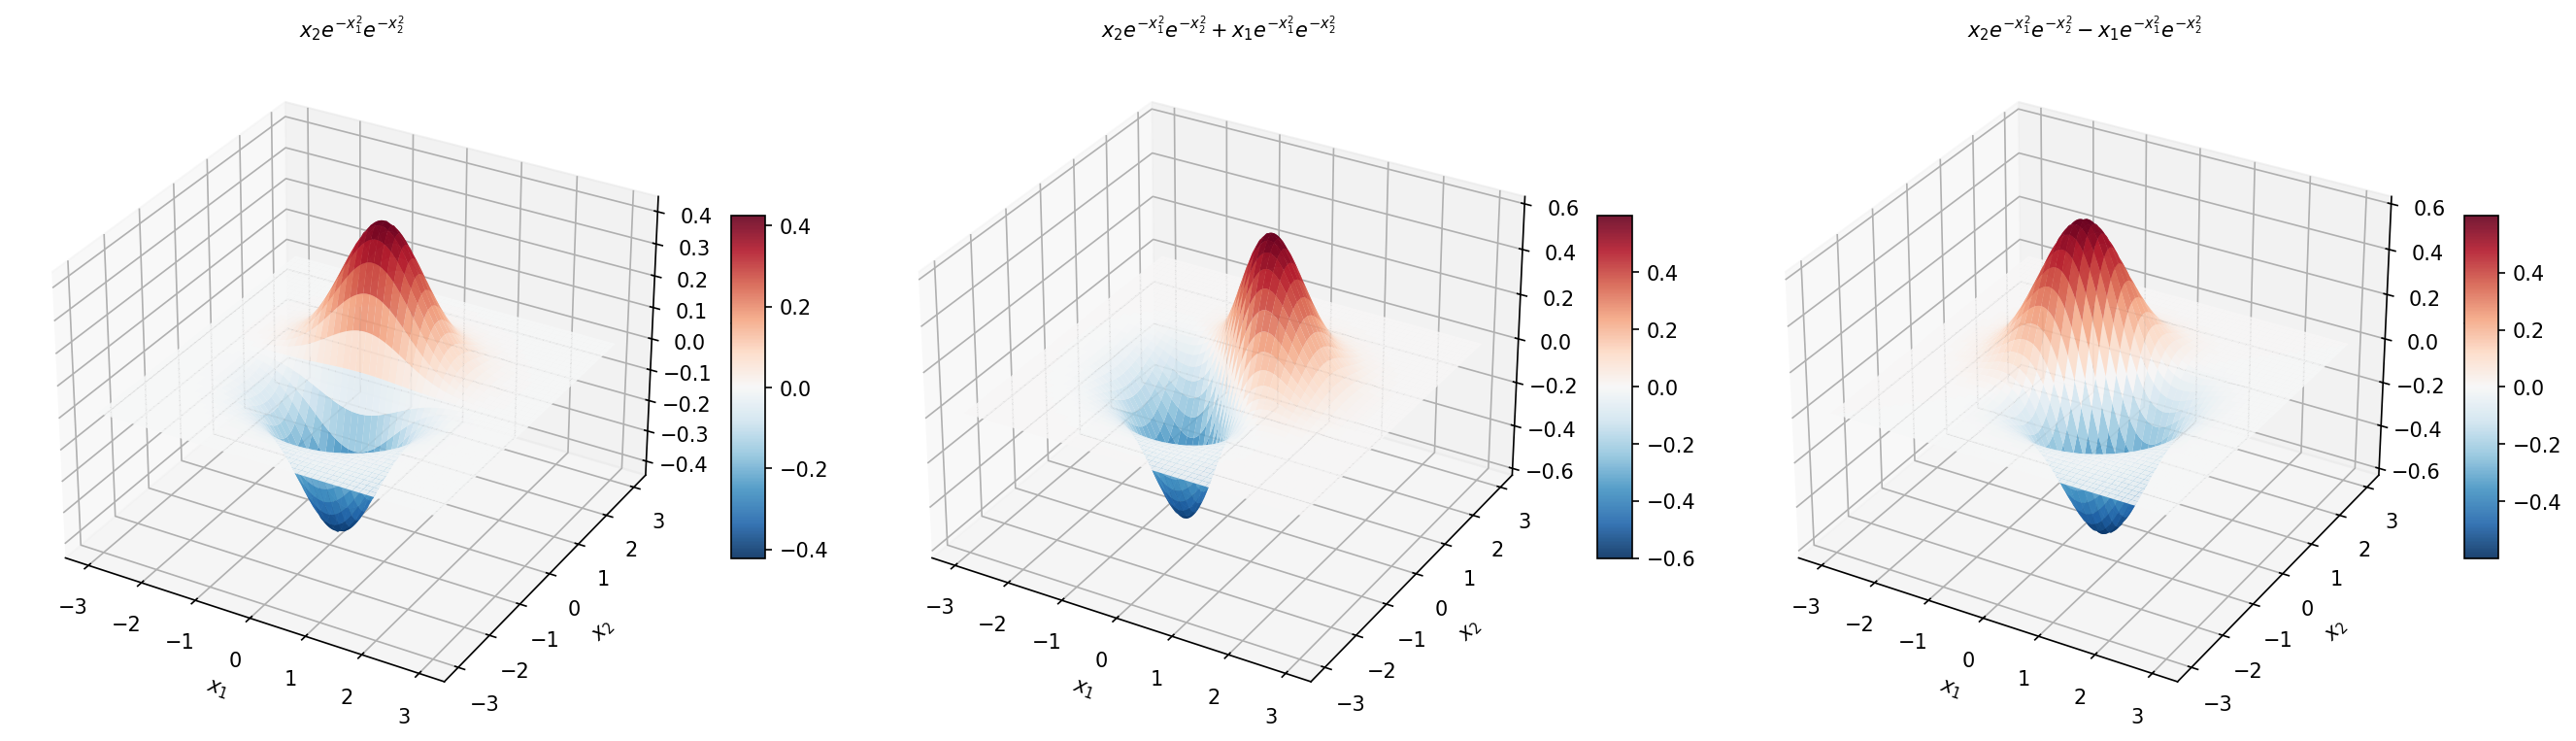
\includegraphics[width=0.8\textwidth,valign=t]{fig/prob5.7_surfaces.png}
        \item 
        $$
        \langle x^2\rangle_0 = \frac{\hbar}{2m\omega}
        $$
        $$
        \langle x^2\rangle_1 = \frac{3\hbar}{2m\omega}
        $$
        \begin{align*}
            \langle x\rangle_{01}=
            &\left(
        \frac{m\omega}{\pi\hbar}
        \right)^{1/2}
        \sqrt{\frac{2m\omega}{\hbar}}
            \int_{-\infty}^\infty
            x^2
        e^{-\frac{m\omega}{\hbar}x^2}
        dx
        \\
        =&
        \left(
        \frac{m\omega}{\pi\hbar}
        \right)^{1/2}
        \sqrt{\frac{2m\omega}{\hbar}}
        \frac{1}{2}
        \sqrt{\frac{\pi}{(\frac{m\omega}{\hbar})^3}}\\
        =&\sqrt{\frac{\hbar}{2m\omega}}
        \end{align*}
        Distinguishable 
        $$
        \langle(x_1-x_2)^2\rangle
        =\frac{2\hbar}{m\omega}
        $$
        Bosons 
        $$
        \langle(x_1-x_2)^2\rangle
        =\frac{\hbar}{m\omega}
        $$
        Fermions 
        $$
        \langle(x_1-x_2)^2\rangle
        =\frac{3\hbar}{m\omega}
        $$
        \item 
        $x_1=R+\frac{1}{2}r,$ $x_2=R-\frac{1}{2}r$
        
        Distinguishable:
        $$
        \frac{m\omega}{\pi\hbar}
        \frac{2m\omega}{\hbar}
        x_2^2
        e^{-\frac{m\omega}{\hbar}x_1^2}
        e^{-\frac{m\omega}{\hbar}x_2^2}
        =
        \frac{2m^2\omega^2}{\pi\hbar^2}
        (R-\frac{1}{2}r)^2
        e^{-\frac{m\omega}{\hbar}(2R^2+\frac{1}{2}r^2)}
        $$
        \begin{align*}
            P(|r|)
        =&
        2\frac{2m^2\omega^2}{\pi\hbar^2}
        \int_{-\infty}^\infty
        (R-\frac{1}{2}r)^2
        e^{-\frac{m\omega}{\hbar}(2R^2+\frac{1}{2}r^2)}dR\\
        =&
        \frac{4m^2\omega^2}{\pi\hbar^2}
        e^{-\frac{m\omega r^2}{2\hbar}}
        \left(\frac{1}{2}\sqrt{\frac{\pi}{(\frac{2m\omega}{\hbar})^3}}
        +\frac{1}{4}r^2
        \sqrt{\frac{\pi}{\frac{2m\omega}{\hbar}}}
        \right)
        \end{align*}
        Bosons:
        \begin{align*}
            &\frac{1}{2}
        \frac{m\omega}{\pi\hbar}
        \frac{2m\omega}{\hbar}
        \left[
        x_2
        e^{-\frac{m\omega}{2\hbar}x_1^2}
        e^{-\frac{m\omega}{2\hbar}x_2^2}
        +
        x_1
        e^{-\frac{m\omega}{2\hbar}x_1^2}
        e^{-\frac{m\omega}{2\hbar}x_2^2}
        \right]^2\\
        =&
        \frac{m^2\omega^2}{\pi\hbar^2}
        4R^2
        e^{-\frac{m\omega}{\hbar}(2R^2+\frac{1}{2}r^2)}
        \end{align*}
        \begin{align*}
            P(|r|)
            =&
            \frac{8m^2\omega^2}{\pi\hbar^2}
        e^{-\frac{m\omega r^2}{2\hbar}}
        \int_{-\infty}^{\infty}
        R^2
        e^{-\frac{m\omega}{\hbar}2R^2}dR\\
        =&
        \frac{4m^2\omega^2}{\pi\hbar^2}
        e^{-\frac{m\omega r^2}{2\hbar}}
        \sqrt{\frac{\pi}{(\frac{2m\omega}{\hbar})^3}}
        \end{align*}
        Fermions:
        \begin{align*}
            &\frac{1}{2}
        \frac{m\omega}{\pi\hbar}
        \frac{2m\omega}{\hbar}
        \left[
        x_2
        e^{-\frac{m\omega}{2\hbar}x_1^2}
        e^{-\frac{m\omega}{2\hbar}x_2^2}
        -
        x_1
        e^{-\frac{m\omega}{2\hbar}x_1^2}
        e^{-\frac{m\omega}{2\hbar}x_2^2}
        \right]^2\\
        =&
        \frac{m^2\omega^2}{\pi\hbar^2}
        r^2
        e^{-\frac{m\omega}{\hbar}(2R^2+\frac{1}{2}r^2)}
        \end{align*}
        \begin{align*}
            P(|r|)
            =&
            \frac{2m^2\omega^2}{\pi\hbar^2}
        e^{-\frac{m\omega r^2}{2\hbar}}
        r^2
        \int_{-\infty}^{\infty}
        e^{-\frac{m\omega}{\hbar}2R^2}dR\\
        =&
        \frac{2m^2\omega^2}{\pi\hbar^2}
        e^{-\frac{m\omega r^2}{2\hbar}}
        r^2
        \sqrt{\frac{\pi}{\frac{2m\omega}{\hbar}}}
        \end{align*}
        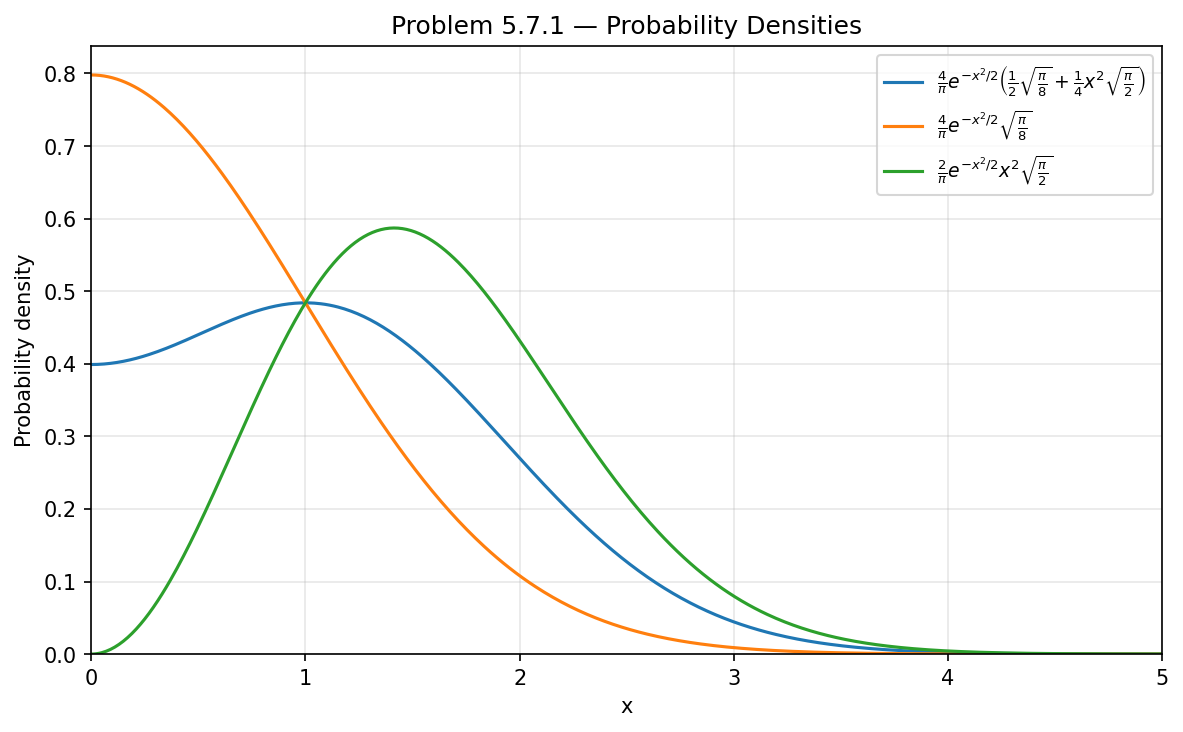
\includegraphics[width=0.8\textwidth,valign=t]{fig/prob5.7.1_densities.png}
    \item 
    Distinguishable:
    \begin{align*}
        \langle n(x)\rangle
        =&
        \frac{m\omega}{\pi\hbar}
        \frac{2m\omega}{\hbar}
        \int_{-\infty}^{\infty}\int_{-\infty}^{\infty}
        (\delta(x-x_1)+\delta(x-x_2))
        x_2^2
        e^{-\frac{m\omega}{\hbar}x_1^2}
        e^{-\frac{m\omega}{\hbar}x_2^2}dx_1dx_2\\
        =&
        \frac{2m^2\omega^2}{\pi\hbar^2}
        e^{-\frac{m\omega x^2}{\hbar}}
        \left[\int
        x_2^2e^{-\frac{m\omega}{\hbar}x_2^2}
        dx_2
        +
        \int
        x^2e^{-\frac{m\omega}{\hbar}x_1^2}
        dx_1
        \right]
        \\
        =&
        \frac{2m^2\omega^2}{\pi\hbar^2}
        e^{-\frac{m\omega x^2}{\hbar}}
        \left[
        \frac{1}{2}
        \sqrt{\frac{\pi}{(\frac{m\omega}{\hbar})^3}}
        +x^2
        \sqrt{\frac{\pi}{\frac{m\omega}{\hbar}}}
        \right]
    \end{align*}
    Bosons:
    \begin{align*}
        \langle n(x)\rangle=&
        \frac{1}{2}
        \frac{m\omega}{\pi\hbar}
        \frac{2m\omega}{\hbar}
        \int
        (\delta(x-x_1)+\delta(x-x_2))
        \left[
        x_2
        e^{-\frac{m\omega}{2\hbar}x_1^2}
        e^{-\frac{m\omega}{2\hbar}x_2^2}
        +
        x_1
        e^{-\frac{m\omega}{2\hbar}x_1^2}
        e^{-\frac{m\omega}{2\hbar}x_2^2}
        \right]^2dx_1dx_2\\
        =&
        \frac{m^2\omega^2}{\pi\hbar^2}
        \int
        (\delta(x-x_1)+\delta(x-x_2))e^{-\frac{m\omega}{\hbar}(x_1^2+x_2^2)}
        (x_1^2+2x_1x_2+x_2^2)dx_1dx_2\\
        =&
        \frac{m^2\omega^2}{\pi\hbar^2}
        \left[
        \int 
        e^{-\frac{m\omega}{\hbar}(x^2+x_2^2)}
        (x^2+2xx_2+x_2^2)dx_2
        +
        \int
        e^{-\frac{m\omega}{\hbar}(x_1^2+x^2)}
        (x_1^2+2x_1x+x^2)dx_1
        \right]\\
        =&
        \frac{m^2\omega^2}{\pi\hbar^2}
        e^{-\frac{m\omega x^2}{\hbar}}
        2\left[x^2\sqrt{\frac{\pi}{\frac{m\omega}{\hbar}}}
        +
        \frac{1}{2}
        \sqrt{\frac{\pi}{(\frac{m\omega}{\hbar})^3}}
        \right]
    \end{align*}
    Fermions:
    \begin{align*}
        \langle n(x)\rangle=&
        \frac{1}{2}
        \frac{m\omega}{\pi\hbar}
        \frac{2m\omega}{\hbar}
        \int
        (\delta(x-x_1)+\delta(x-x_2))
        \left[
        x_2
        e^{-\frac{m\omega}{2\hbar}x_1^2}
        e^{-\frac{m\omega}{2\hbar}x_2^2}
        -
        x_1
        e^{-\frac{m\omega}{2\hbar}x_1^2}
        e^{-\frac{m\omega}{2\hbar}x_2^2}
        \right]^2dx_1dx_2\\
        =&
        \frac{m^2\omega^2}{\pi\hbar^2}
        \int
        (\delta(x-x_1)+\delta(x-x_2))e^{-\frac{m\omega}{\hbar}(x_1^2+x_2^2)}
        (x_1^2-2x_1x_2+x_2^2)dx_1dx_2\\
        =&
        \frac{m^2\omega^2}{\pi\hbar^2}
        \left[
        \int 
        e^{-\frac{m\omega}{\hbar}(x^2+x_2^2)}
        (x^2-2xx_2+x_2^2)dx_2
        +
        \int
        e^{-\frac{m\omega}{\hbar}(x_1^2+x^2)}
        (x_1^2-2x_1x+x^2)dx_1
        \right]\\
        =&
        \frac{m^2\omega^2}{\pi\hbar^2}
        e^{-\frac{m\omega x^2}{\hbar}}
        2\left[x^2\sqrt{\frac{\pi}{\frac{m\omega}{\hbar}}}
        +
        \frac{1}{2}
        \sqrt{\frac{\pi}{(\frac{m\omega}{\hbar})^3}}
        \right]
    \end{align*}
    All three expected density operators are the same.
    
    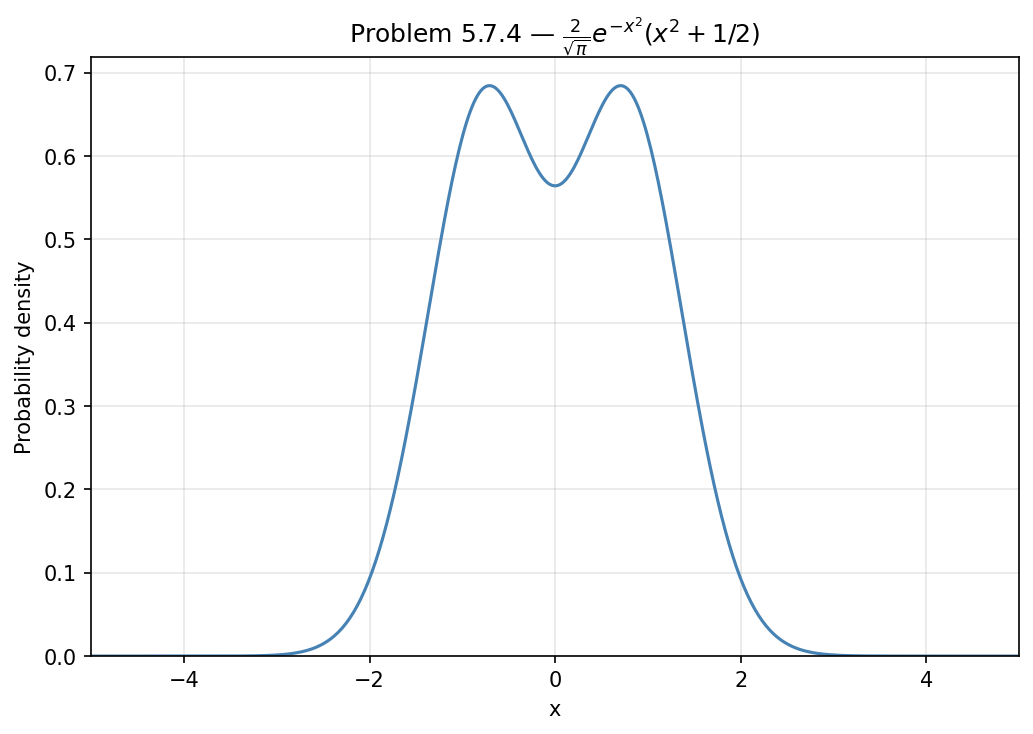
\includegraphics[width=0.8\textwidth,valign=t]{fig/prob5.7.4_density.png}
   \end{enumerate}
   \subsection*{Sol. 8}
   Distinguishable
   $$
   \psi_a(x_1)\psi_b(x_2)\psi_c(x_3)
   $$
   Bosons
   \begin{align*}
       &\psi_a(x_1)\psi_b(x_2)\psi_c(x_3) + 
       \psi_a(x_1)\psi_b(x_3)\psi_c(x_2) + 
       \psi_a(x_2)\psi_b(x_1)\psi_c(x_3)\\
       &+ 
       \psi_a(x_2)\psi_b(x_3)\psi_c(x_1) + 
       \psi_a(x_3)\psi_b(x_1)\psi_c(x_2)+ 
       \psi_a(x_3)\psi_b(x_2)\psi_c(x_1)
   \end{align*}
   Fermions
   \begin{align*}
       \begin{vmatrix}
       \psi_a(x_1) & \psi_b(x_1) & \psi_c(x_1)\\
       \psi_a(x_2) & \psi_b(x_2) & \psi_c(x_2)\\
       \psi_a(x_3) & \psi_b(x_3) & \psi_c(x_3)\\
       \end{vmatrix}=
       &\psi_a(x_1)\psi_b(x_2)\psi_c(x_3) + 
       \psi_a(x_3)\psi_b(x_1)\psi_c(x_2) + 
       \psi_a(x_2)\psi_b(x_3)\psi_c(x_1)\\
       &- 
       \psi_a(x_3)\psi_b(x_2)\psi_c(x_1) -
       \psi_a(x_2)\psi_b(x_1)\psi_c(x_3)-
       \psi_a(x_1)\psi_b(x_3)\psi_c(x_2)
   \end{align*}


   \subsection*{Sol. 9}
   \begin{enumerate}
       \item 
       The four lowest energy configuration for the infinite square well is 
   $$
   \psi_{11}|00\rangle,\;E=2K,\; d=1
   $$
   $$
   (\psi_{12}-\psi_{21})|11\rangle,\;
   (\psi_{12}-\psi_{21})|10\rangle,\;
   (\psi_{12}-\psi_{21})|1-1\rangle,\;
   (\psi_{12}+\psi_{21})|00\rangle
   E=5K,\;d=4
   $$
   $$
   \psi_{22}|00\rangle,\;
   E=8K,\;d=1
   $$
   $$
   (\psi_{13}-\psi_{31})|11\rangle,\;
   (\psi_{13}-\psi_{31})|10\rangle,\;
   (\psi_{13}-\psi_{31})|1-1\rangle,\;
   (\psi_{13}+\psi_{31})|00\rangle.\;
   E=10K,\;d=4
   $$
   \item 
   Note that the particle is a boson. By the CB table,
   the symmetric configurations are 
   $$
   |22\rangle, |21\rangle, |20\rangle, |00\rangle, |2-1\rangle, |2-2\rangle,
   $$
   and the anti-symmetric configurations are
   $$
   |11\rangle, |10\rangle, |1-1\rangle.
   $$

   The degeneracies for $2K$ is $6,$ 
   for $5K$ is $9,$ 
   for $8K$ is $6,$ 
   for $10K$ is $9.$ 
   \end{enumerate}
   \subsection*{Sol. 10}
   \begin{enumerate}
       \item By doing the anti-symmetry under 1 and 2,
       we have $a=b=g=h=0,$ and 
       $c=-e,$ $d=-f.$ Now we changes 2 and 3,
       we have $e=0=c,$ $d=0=f.$ Thus, such anti-symmetric configuration is impossible.
       \item The ground state energy is $6K$
       \begin{align*}
           &\begin{vmatrix}
               \psi_1(x_1)|\uparrow\rangle_1 & 
               \psi_1(x_1)|\downarrow\rangle_1 & 
               \psi_2(x_1)|\uparrow\rangle_1\\
               \psi_1(x_2)|\uparrow\rangle_2 & 
               \psi_1(x_2)|\downarrow\rangle_2 & 
               \psi_2(x_2)|\uparrow\rangle_2\\
               \psi_1(x_3)|\uparrow\rangle_3 & 
               \psi_1(x_3)|\downarrow\rangle_3 & 
               \psi_2(x_3)|\uparrow\rangle_3\\
           \end{vmatrix}\\
           =&
    \psi_1(x_1)\psi_1(x_2)\psi_2(x_3)|\uparrow\downarrow\uparrow\rangle
    +
    \psi_1(x_1)\psi_2(x_2)\psi_1(x_3)|\downarrow\uparrow\uparrow\rangle+
    \psi_2(x_1)\psi_1(x_2)\psi_1(x_3)|\uparrow\uparrow\downarrow\rangle
    \\&-
    \psi_2(x_1)\psi_1(x_2)\psi_1(x_3)|\uparrow\downarrow\uparrow\rangle
    -
    \psi_1(x_1)\psi_1(x_2)\psi_2(x_3)|\downarrow\uparrow\uparrow\rangle-
    \psi_1(x_1)\psi_2(x_2)\psi_1(x_3)|\uparrow\uparrow\downarrow\rangle
       \end{align*}
       \begin{align*}
           &\begin{vmatrix}
               \psi_1(x_1)|\uparrow\rangle_1 & 
               \psi_1(x_1)|\downarrow\rangle_1 & 
               \psi_2(x_1)|\downarrow\rangle_1\\
               \psi_1(x_2)|\uparrow\rangle_2 & 
               \psi_1(x_2)|\downarrow\rangle_2 & 
               \psi_2(x_2)|\downarrow\rangle_2\\
               \psi_1(x_3)|\uparrow\rangle_3 & 
               \psi_1(x_3)|\downarrow\rangle_3 & 
               \psi_2(x_3)|\downarrow\rangle_3\\
           \end{vmatrix}\\
           =&
    \psi_1(x_1)\psi_1(x_2)\psi_2(x_3)|\uparrow\downarrow\downarrow\rangle
    +
    \psi_1(x_1)\psi_2(x_2)\psi_1(x_3)|\downarrow\downarrow\uparrow\rangle+
    \psi_2(x_1)\psi_1(x_2)\psi_1(x_3)|\downarrow\uparrow\downarrow\rangle
    \\&-
    \psi_2(x_1)\psi_1(x_2)\psi_1(x_3)|\downarrow\downarrow\uparrow\rangle
    -
    \psi_1(x_1)\psi_1(x_2)\psi_2(x_3)|\downarrow\uparrow\downarrow\rangle-
    \psi_1(x_1)\psi_2(x_2)\psi_1(x_3)|\uparrow\downarrow\downarrow\rangle
       \end{align*}
       The degeneracy is 2.
       \item 
       \begin{align*}
           &\psi_1(x_1)\psi_1(x_2)\psi_2(x_3)|\uparrow\downarrow\uparrow\rangle
    +
    \psi_1(x_1)\psi_2(x_2)\psi_1(x_3)|\downarrow\uparrow\uparrow\rangle+
    \psi_2(x_1)\psi_1(x_2)\psi_1(x_3)|\uparrow\uparrow\downarrow\rangle
    \\&-
    \psi_2(x_1)\psi_1(x_2)\psi_1(x_3)|\uparrow\downarrow\uparrow\rangle
    -
    \psi_1(x_1)\psi_1(x_2)\psi_2(x_3)|\downarrow\uparrow\uparrow\rangle-
    \psi_1(x_1)\psi_2(x_2)\psi_1(x_3)|\uparrow\uparrow\downarrow\rangle\\
    =&\psi_1(x_1)\psi_1(x_2)
    (|\uparrow\downarrow\rangle -|\downarrow\uparrow\rangle)\psi_2(x_3)|\uparrow\rangle\\
    &
    +\psi_1(x_1)\psi_1(x_3)
    (-|\uparrow\downarrow\rangle_{13} +|\downarrow\uparrow\rangle_{13})\psi_2(x_3)|\uparrow\rangle_{2}
    +
    \psi_1(x_2)\psi_1(x_3)
    (|\uparrow\downarrow\rangle_{23} -|\downarrow\uparrow\rangle_{23})\psi_2(x_1)|\uparrow\rangle_{1}\\
    =&\Phi(1,2)\phi(3) -\Phi(1,3)\phi(2) + \Phi(2,3)\phi(1)
       \end{align*}
   \end{enumerate}
   \subsection*{Sol. 11}
   \begin{enumerate}
       \item Trivial
       \item 
       For $q=1,$ $N=3,$
       \begin{align*}
           \psi(z_1,z_2,z_3)
           =&
           A\left[
           (z_1-z_2)(z_1-z_3)(z_2-z_3)
           \right]
           \exp\left[
           -\frac{1}{2}
           (|z_1|^2+|z_2|^2+|z_3|^2)
           \right]\\
           =&
           A[z_1^2z_2-z_1^2z_3+z_1z_3^2-z_1z_2^2+z_2^2z_3-z_2z_3^2]
           \exp\left[
           -\frac{1}{2}
           (|z_1|^2+|z_2|^2+|z_3|^2)
           \right]\\
           =&
           A
           \begin{vmatrix}
           z_1^2e^{-\frac{1}{2}|z_1|^2} & z_1e^{-\frac{1}{2}|z_1|^2} & e^{-\frac{1}{2}|z_1|^2}\\
           z_2^2e^{-\frac{1}{2}|z_2|^2} & z_2e^{-\frac{1}{2}|z_2|^2} & e^{-\frac{1}{2}|z_2|^2}\\
           z_3^2e^{-\frac{1}{2}|z_3|^2} & z_3e^{-\frac{1}{2}|z_3|^2} & e^{-\frac{1}{2}|z_3|^2}\\
       \end{vmatrix}
       \end{align*}
       The states in which a single particle is occupied are $z^2e^{-\frac{1}{2}|z|^2},$
       $ze^{-\frac{1}{2}|z|^2},$ $e^{-\frac{1}{2}|z|^2}.$
       \item 
       For $q=3,$ $N=2,$
       \begin{align*}
           \psi(z_1,z_2,z_3)
           =&
           A
           (z_1-z_2)^3
           \exp\left[
           -\frac{1}{2}
           (|z_1|^2+|z_2|^2)
           \right]\\
           =&
           A[z_1^3-3z_1^2z_2+3z_1z_2^2-z_2^3]
           \exp\left[
           -\frac{1}{2}
           (|z_1|^2+|z_2|^2)
           \right]\\
           =&
           A
           \begin{vmatrix}
           z_1^3e^{-\frac{1}{2}|z_1|^2} & e^{-\frac{1}{2}|z_1|^2} \\
           z_2^3e^{-\frac{1}{2}|z_2|^2} & e^{-\frac{1}{2}|z_2|^2} 
       \end{vmatrix}
       +A
       \begin{vmatrix}
           -3z_1^2e^{-\frac{1}{2}|z_1|^2} & z_1e^{-\frac{1}{2}|z_1|^2} \\
           3z_2^2e^{-\frac{1}{2}|z_2|^2} & z_2e^{-\frac{1}{2}|z_2|^2} 
       \end{vmatrix}
       \end{align*}
       
       
   \end{enumerate}

   \subsection*{Sol. 12}
   \begin{enumerate}
       \item Note the Hamiltonian is symmetric in any $r,$ so any permutation of the arguments in the solution satisfies the equation. A completely symmetric function can then be constructed by adding all the $Z!$ terms together. For the anti-symmetry function, change the plus sign to a minus sign for any transposition(changing two labels only) it has done.

        If $\psi$ is symmetric in the first two terms, all the terms, fixing the third to the last terms, are canceled. For any $Z!$ terms, there is a term to let it get canceled, therefore, if any two terms are symmetric, the anti-symmetric function is not able to be construed.
        \item 
        There are only two possible spin states for an electron, by the pigeon hole principle, if $Z>2,$ there will be two electrons occupied in the same spin state, and is thus symmetric. By the argument above, there is no way to construct an anti-symmetry configuration.
        
   \end{enumerate}

   \subsection*{Sol. 13}
   \begin{enumerate}
       \item The total energy of two $n=2$ electrons is 
       $$
       4(-\frac{13.6}{4}-\frac{13.6}{4})=-27.2.
       $$
       The energy of the emitted electron would be 
       $$
       -27.2 - (-13.6)\times 4 = 27.2eV.
       $$
       \item 
       $$
       \frac{1}{\lambda}
       =4\mathcal{R}(\frac{1}{n_f^2}-\frac{1}{n_i^2})
       $$
   \end{enumerate}
   \subsection*{Sol. 14}
   \begin{enumerate}
       \item 
       For the ground state
       $$
       \psi_{100}(r_1)\psi_{100}(r_2),
       $$
       paired with a triplet configuration.
        For the excited state
       $$
       \psi_{nlm}(r_1)\psi_{100}(r_2)\pm \psi_{nlm}(r_2)\psi_{100}(r_1),
       $$
       paired with a triplet configuration if plus, and a singlet if minus.
        The energy level scheme is therefore $4(E_1+E_1)$ for the ground state, which is non-degenerate, and is $4(E_n+E_1)$ for the excited states, each having four degeneracies.
       \item  If those electrons are distinguishable, the energy schema would be $4(E_n+E_1),$ each having four degeneracies.
       
   \end{enumerate}
   \subsection*{Sol. 15}
   \begin{enumerate}
       \item 
       \begin{align*}
           &\int\frac{1}{|\bm r_1-\bm r_2|}
           \frac{64}{\pi^2 a^6}e^{-4(r_1+r_2)/a}d^3\bm r_1 d^3\bm r_2\\
           =&\frac{64}{\pi^2 a^6}
           \int\left[\frac{1}{\sqrt{r_1^2+r_2^2-2r_1r_2\cos\theta_2}} e^{-4r_2/a}r_2^2\sin\theta_2
           dr_2d\theta_2d\phi_2
           \right] e^{-4r_1/a}d^3\bm r_1
       \end{align*}
       \begin{align*}
           &2\pi\int_{0}^{\pi}
           \frac{1}{\sqrt{r_1^2+r_2^2-2r_1r_2\cos\theta_2}} e^{-4r_2/a}r_2^2\sin\theta_2
           d\theta_2\\
           =&
           2\pi e^{-4r_2/a}r_2^2\int_{r_1^2+r_2^2-2r_1r_2}^{r_1^2+r_2^2+2r_1r_2} \frac{1/(2r_1r_2)}{\sqrt{t}}dt\\
           =&2\pi e^{-4r_2/a}\frac{r_2}{r_1}
           \left(\sqrt{r_1^2+r_2^2+2r_1r_2} - \sqrt{r_1^2+r_2^2-2r_1r_2}\right)
       \end{align*}
       \begin{align*}
           &\int_{r_1}^{\infty}
           2\pi e^{-4r_2/a}\frac{r_2}{r_1}
           \left(\sqrt{r_1^2+r_2^2+2r_1r_2} - \sqrt{r_1^2+r_2^2-2r_1r_2}\right) dr_2\\
           =&2\pi\frac{1}{r_1}
           \int_{r_1}^{\infty}
           e^{-4r_2/a}r_2
           ((r_1+r_2)-(r_2-r_1))dr_2\\
        =&4\pi\int_{r_1}^{\infty}r_2e^{-4r_2/a}dr_2\\
        =&4\pi e^{-4r_2/a}\frac{-4/ar_2-1}{16/a^2}\bigg|^{\infty}_{r_1}\\
        =&\pi e^{-4r_1/a}(ar_1+\frac{1}{4}a^2)
       \end{align*}
       \begin{align*}
           &\int_{0}^{r_1}
           2\pi e^{-4r_2/a}\frac{r_2}{r_1}
           \left(\sqrt{r_1^2+r_2^2+2r_1r_2} - \sqrt{r_1^2+r_2^2-2r_1r_2}\right) dr_2\\
           =&2\pi\frac{1}{r_1}
           \int_{0}^{r_1}
           e^{-4r_2/a}r_2
           ((r_1+r_2)-(r_1-r_2))dr_2\\
        =&4\pi\frac{1}{r_1}\int_{0}^{r_1}r_2^2e^{-4r_2/a}dr_2\\
        =&4\pi\frac{1}{r_1} 
        e^{-4r_2/a}(\frac{r_2^2}{-4/a}-\frac{2r_2}{16/a^2}+\frac{2}{-64/a^3})\bigg|^{r_1}_{0}\\
        =&
        4\pi\frac{1}{r_1} 
        \left[e^{-4r_1/a}(\frac{r_1^2}{-4/a}-\frac{2r_1}{16/a^2}+\frac{2}{-64/a^3})
        -\frac{2}{-64/a^3}
        \right]\\
        =&\pi(e^{-4r_1/a}(-r_1a-\frac{1}{2}a^2-\frac{a^3}{8r_1})+\frac{a^3}{8r_1})
       \end{align*}
       \begin{align*}
           &\frac{64}{\pi^2 a^6}
           \int\left[
           \pi e^{-4r_1/a}(ar_1+\frac{1}{4}a^2)
           +
           \pi(e^{-4r_1/a}(-r_1a-\frac{1}{2}a^2-\frac{a^3}{8r_1})+\frac{a^3}{8r_1})
           \right]e^{-4r_1/a}r_1^2\sin\theta_1 dr_1d\theta_1d\phi_1\\
           =&
           \frac{64}{ a^6}4
           \int 
           \left[
           (e^{-4r_1/a}(-\frac{1}{4}a^2-\frac{a^3}{8r_1})+\frac{a^3}{8r_1})
           \right]e^{-4r_1/a}r_1^2 dr_1\\
           =&
           \frac{64}{ a^6}4
           \int 
           \left[
           -\frac{1}{4}e^{-8r_1/a}a^2r_1^2 
            -\frac{1}{8}e^{-8r_1/a}a^3r_1
            +\frac{1}{8}e^{-4r_1/a}a^3r_1
           \right] dr_1\\
           =&
           \frac{256}{a^6}
           \bigg[
           -\frac{1}{4}a^2
           e^{-8/ar_1}
           (\frac{r_1^2}{-8/a}-\frac{2r_1}{64/a^2}+\frac{2}{-512/a^3})
           \bigg|^\infty_0\\
           &-
           \frac{1}{8}
           a^3
           e^{-8/ar_1}(\frac{-8/ar_1-1}{64/a^2})
           \bigg|^\infty_0
           +\frac{1}{8}
           a^3e^{-4/ar_1}(\frac{-4/ar_1-1}{16/a^2})\bigg|^\infty_0
           \bigg]\\
           =&
           \frac{256}{a^6}
           \left[
           -a^2\frac{a^3}{1024}
           -a^3\frac{a^2}{512}
           +a^3\frac{a^2}{128}
           \right]=\frac{5}{4a}
       \end{align*}
       \item 
       The estimated repulsion energy is 
       $$
       \frac{1}{4\pi\epsilon_0}\frac{5e^2}{4a}\approx 
       34eV,
       $$
       approximately meets the gap between $-109eV$ to $-79eV.$
       
   \end{enumerate}

   \subsection*{Sol. 16}
   The energy of this state is 
   $$
   -13.6\times9\times 2 + (-13.6\times 9 / 4)
   = -275.4
   $$
   By problem 5.10, there are two degeneracies for this configuration.

   \subsection*{Sol. 17}
   \begin{enumerate}
       \item 
       H: $(1s)$

   He: $(1s)^2$

   Li: $(1s)^2(2s)$

   Be: $(1s)^2(2s)^2$

   B: $(1s)^2(2s)^2(2p)$

   C: $(1s)^2(2s)^2(2p)^2$

   N: $(1s)^2(2s)^2(2p)^3$

   O: $(1s)^2(2s)^2(2p)^4$

   F: $(1s)^2(2s)^2(2p)^5$

   Ne: $(1s)^2(2s)^2(2p)^6$

   \item 

   H: $ \prescript{2}{}{S}_{1/2} $

   He: $ \prescript{1}{}{S}_{0} $

   Li: $ \prescript{2}{}{S}_{1/2} $

   Be: $ \prescript{1}{}{S}_{0} $

   For Boron, the total orbital momenta could be $1,$ and the total spin momenta could be $\frac{1}{2},$ so the total momenta could be $\frac{3}{2}$ or $\frac{1}{2}.$

   For Carbon, the total orbital momenta could be $2,$ $1$ or $0,$ and the total spin momenta could be $1,$ or $0$ so the total momenta could be $3$, $2,$ $1$ or $0.$

    For Nitrogen, the total orbital momenta could be $3,$ $2,$ $1$ or $0,$ and the total spin momenta could be $\frac{3}{2},$ or $\frac{1}{2}$ so the total momenta could be $\frac{5}{2}$, $\frac{3}{2},$ or $\frac{1}{2}.$
   
   \end{enumerate}

   \subsection*{Sol. 18}
   \begin{enumerate}
       \item The excited states would be orthohelium, namely, a triplet configuration.
       \item 
       The Hund's first rule favors $S=1,$ which is symmetric, so the orbital state should be anti symmetric. $L=2$ is symmetric, so it will be $S=1,$ $L=1.$
       \item 
       Boron is no more than half filled, so $J=\frac{1}{2}.$
       \item 
       For Carbon, $S=1,$ $L=1,$ and it is no more than half filled, therefore $J=0.$

       For Nitrogen, $S=\frac{3}{2}.$
        From Slater's determinant: 
        \begin{align*}
            \begin{vmatrix}
                |11\rangle_1 & |10\rangle_1 & |1-1\rangle_1\\
                |11\rangle_2 & |10\rangle_2 & |1-1\rangle_2\\
                |11\rangle_3 & |10\rangle_3 & |1-1\rangle_3\\
            \end{vmatrix}
            =&|11\rangle_1|10\rangle_2|1-1\rangle_3
            +
            |10\rangle_1|1-1\rangle_2|11\rangle_3
            +|1-1\rangle_1|11\rangle_2|10\rangle_3\\
            &-|1-1\rangle_1|10\rangle_2|11\rangle_3
            -|10\rangle_1|11\rangle_2|1-1\rangle_3
            -|11\rangle_1|1-1\rangle_2|10\rangle_3,
        \end{align*}
        note that the anti-symmetric subspace is one-dimensional, thus
        restricting the possibility to the state $|00\rangle,$ so
       $L=0.$ It is no more than half filled, therefore $J=\frac{3}{2}.$

        
       
   \end{enumerate}
   \subsection*{Sol. 19}
   The total spin is $2,$ total orbital momenta is $6,$ and the grand total angular momenta is $8.$

   $$
   (1s)^2(2s)^2(2p)^6(3s)^2(3p)^6(3d)^{10}(4s)^2(4p)^6
   (4d)^{10}(5s)^2(5p)^6(4f)^{10}(6s)^2
   $$
   \subsection*{Sol. 20}
   \begin{align*}
       \frac{E_{tot}}{Nd}=
       \frac{\hbar^2(3\pi^2Nd)^{5/3}}{10\pi^2mNd}V^{-2/3}
   \end{align*}
   \begin{align*}
       E_F = \frac{\hbar^2}{2m}(3\rho\pi^2)^{2/3}
       =\frac{\hbar^2}{2m}(3\frac{Nd}{V}\pi^2)^{2/3}
   \end{align*}
   \begin{align*}
       \frac{E_{tot}}{NdE_F}
       =
       \frac{3}{5}
   \end{align*}

   \subsection*{Sol. 21}
   \begin{enumerate}
       \item 
       \begin{align*}
           E_F=&\frac{\hbar^2}{2m}(3\rho\pi^2)^{2/3}
           =\frac{(1.054\times10^{-34})^2}{2\times9.109\times10^{-31}}
           (3\frac{8.96/63.5\times 6.022\times10^{23}}{(0.01)^3}\pi^2)^{2/3}
           /(1.602\times 10^{-19}) eV\\
           \approx &7.04eV
       \end{align*}
       \item 
       \begin{align*}
           v = \frac{\hbar}{m}(3\rho\pi^2)^{1/3}\approx 1.57\times 10^6m/s
       \end{align*}
       Pretty safe to assume them to be nonrelativistic.
       \item $$T=81739K.$$
       \item 
       $$
       P = 3.834\times 10^{10}N/m^2.
       $$
   \end{enumerate}

   \subsection*{Sol. 22}
    $$
    E_F=\frac{(1.054\times 10^{-34})^2}
    {2\times3\times 1.66\times10^{-27}}
    (3\times82/(3\times 1.66\times10^{-27})\times\pi^2)^{2/3}
    =6.909\times 10^{-23}J
    $$
    $$
    T = 5K
    $$

   \subsection*{Sol. 23}
   \begin{align*}
       \frac{dP}{dV}
       =-k\frac{5}{3}\rho^{2/3}\frac{Nd}{V^2}
       =-k\frac{5}{3}\rho^{5/3}/V
       =-\frac{5}{3}P/V
   \end{align*}
   $$
   B = -V\frac{dP}{dV}
   =\frac{5}{3}P
   $$
   For copper 
   $$
   B = 6.39\times10^{10}
   $$

   \subsection*{Sol. 24}
   \begin{enumerate}
       \item 
       \begin{align*}
           \psi(x)
           =
           &A\sin(kx) + \frac{A\sin(ka)}{e^{iqa}-\cos(ka)}\cos(kx)\\
           =&
           \frac{A}{e^{iqa}-\cos(ka)}[\sin(kx)e^{iqa}-\sin(kx)\cos(ka)
           +\sin(ka)\cos(kx)]\\
           =&
           \frac{Ae^{iqa}}{e^{iqa}-\cos(ka)}
           [\sin(kx)+e^{-iqa}\sin(k(a-x))]
       \end{align*}
       \item 
       If $z=j\pi,$ 
        by equation 5.68
        $$
        B = e^{-iqa}B(-1)^j,
        $$
        and by equation 5.69
        $$
        kA-e^{-iqa}kA(-1)^j = \frac{2m\alpha}{\hbar^2}B.
        $$
        We must have $B=0,$ or $e^{-iqa}=(-1)^j.$ If $e^{-iqa}=(-1)^j,$ then $B=0,$ so either way $B=0.$
        Thus the wave function is $\psi(x)=\sin(kx).$ At the delta function, $\psi(0)=0.$
   \end{enumerate}

   \subsection*{Sol. 25}
   The lowest allowed $z=2.628,$ note that 
   $$
   E = \frac{\hbar^2k^2}{2m} = \frac{z^2\alpha}{2\beta a} = 0.345 eV.
   $$

   \subsection*{Sol. 26}
   For $E<0,$ 
   all the derivations are the same. By substituting the relation $ik=\kappa$ into equation 5.71, 
   we have 
   \begin{align*}
       \cos(qa) =& \cos(-i\kappa a) + \frac{m\alpha}{-\hbar^2i\kappa}\sin(-i\kappa a)\\
       =& \cos(iz) + \frac{m\alpha a}{\hbar^2i z}\sin(iz)\\
       =&\cosh z + \frac{m\alpha a}{\hbar^2 z}\sinh z\\
       =&\cosh z + \beta\frac{\sinh z}{z}.
   \end{align*}
   
    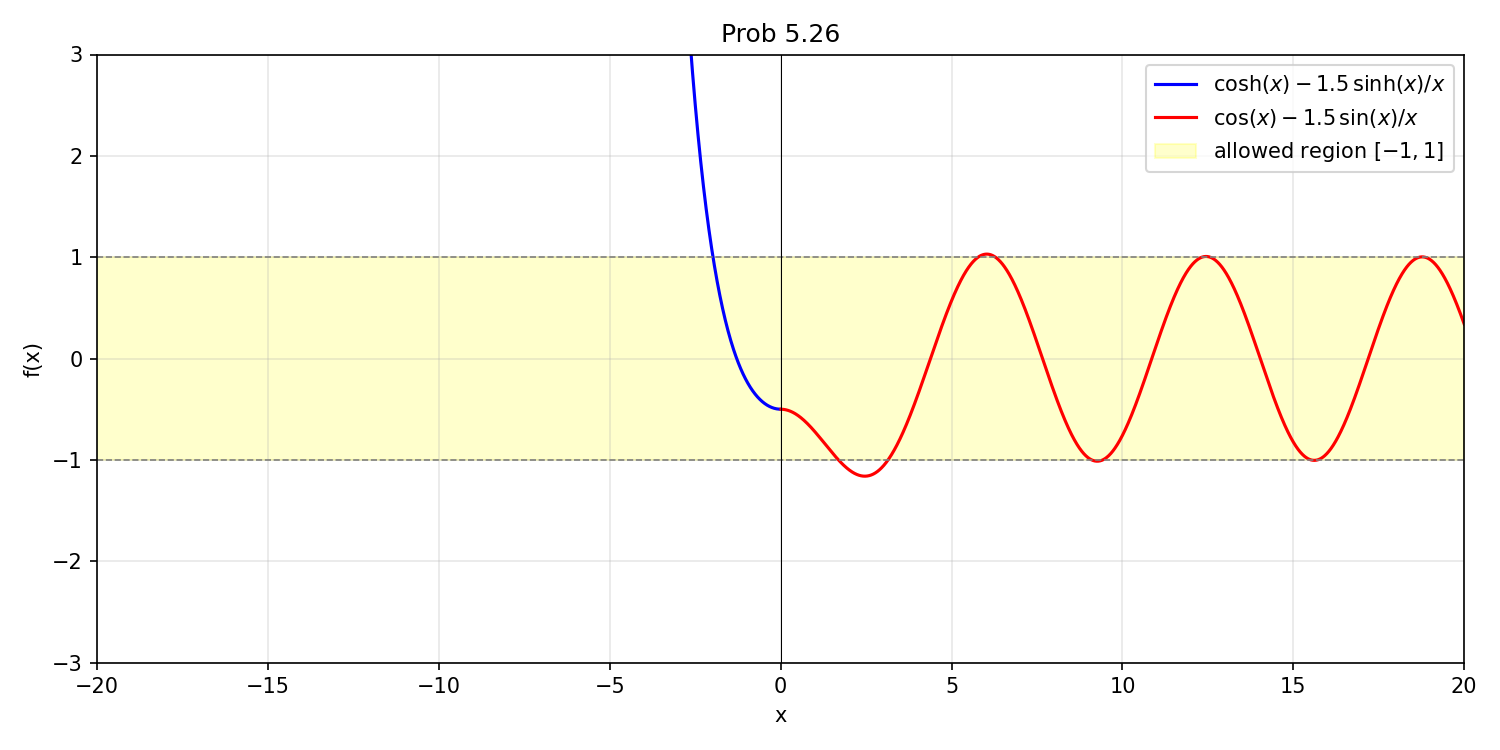
\includegraphics[width=0.8\textwidth,valign=t]{fig/prob5.26.png}
    
   There are $N$ states in the first band. 

   \subsection*{Sol. 27}
   For a given allowed value $k,$ equation 5.71 determines $\cos(qa).$ By recognizing $qa=\frac{2\pi n}{N},$ where $n=0,\dots,N-1$ as the angle of a circle, by symmetry, almost all $\cos(qa)$ corresponds to a pair of $n$s. Except when $\cos(qa)=\pm 1.$

   \subsection*{Sol. 28}
   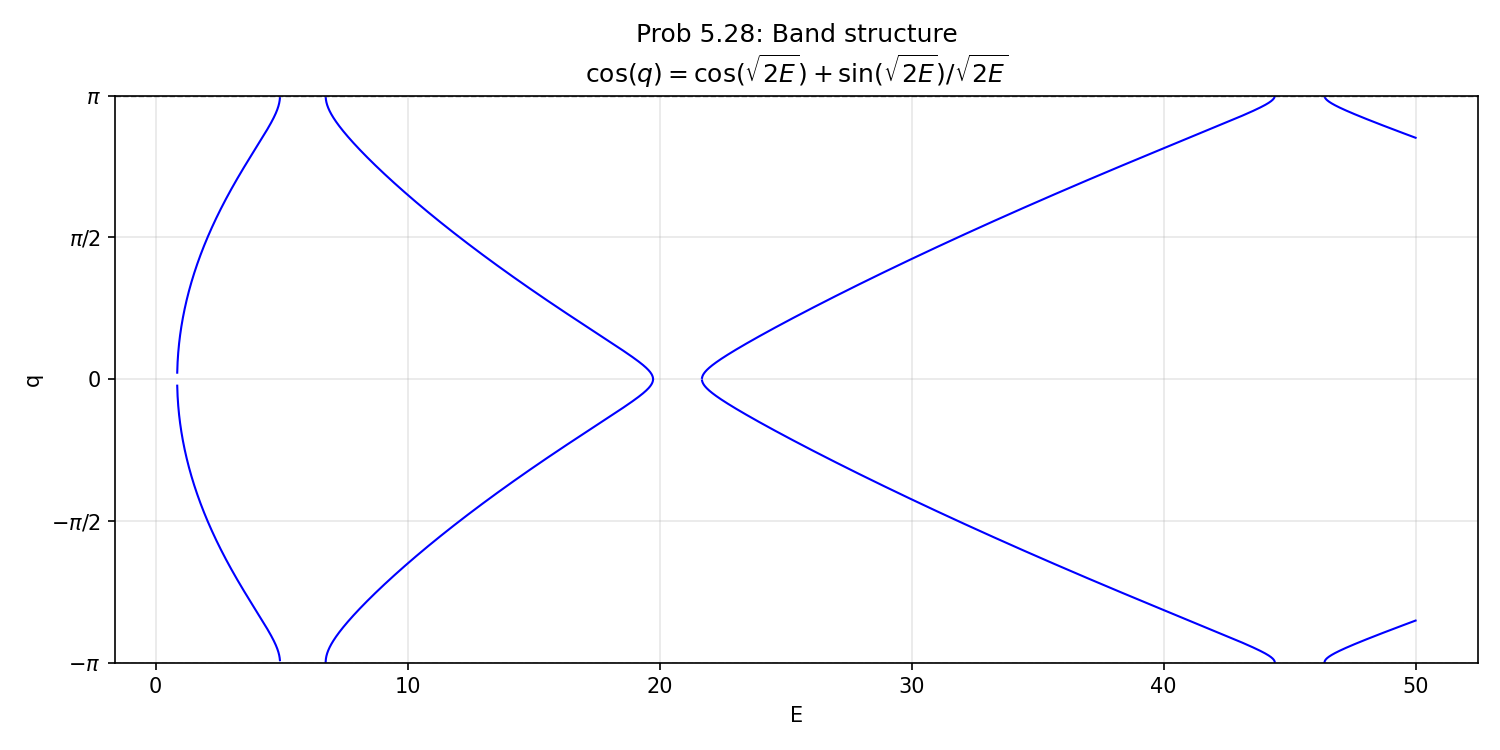
\includegraphics[width=0.8\textwidth,valign=t]{fig/prob5.28.png}

   \subsection*{Sol. 29}
   \begin{enumerate}
       \item 27 states if they are distinguishable.
       \item We can use the permanent method to construct the symmetric states. There would be $3+6+1=10$ possible states for identical bosons.
       \item Only 1 possible state if they are identical fermions.
   \end{enumerate}

   \subsection*{Sol. 30}
   $$
   \frac{1}{4}
   (\pi k_F^2)
   =\frac{Nd}{2}\frac{\pi^2}{A}\Rightarrow
   k_F=\sqrt{2\sigma\pi}
   $$
   $$
   E_F=\frac{\hbar^2\sigma\pi}{m}
   $$

   \subsection*{Sol. 31}
   An electron at the ground state of  a 3-dim infinite square well of width $a$ has energy $\frac{3\pi^2\hbar^2}{2ma^2}.$ So the total energy of $N$ isolated electrons is $\frac{3N\pi^2\hbar^2}{2ma^2}.$

   By equation 5.56, the total energy of all the filled state in a 3-dim square well of width $N^{1/3}a$ is 
   $$
   E=\frac{\hbar^2(3\pi^2N)^{5/3}}{10\pi^2m}(Na^3)^{-2/3}
   $$

   The cohesive energy per atom is thus 
   \begin{align*}
       \frac{3\pi^2\hbar^2}{2ma^2} - 
       \frac{\hbar^2(3\pi^2)^{5/3}}{10\pi^2ma^2}
       =&
       \frac{3\pi^2\hbar^2}{2ma^2}
       \left(1-\frac{3^{2/3}}{5\pi^{2/3}}\right).
   \end{align*}
    

   \subsection*{Sol. 32}
   \begin{enumerate}
       \item 
       \begin{align*}
       E_{tot}=\frac{1}{2}\frac{\hbar^2(3\pi^2 2N_+)^{5/3}}{10\pi^2m}V^{-2/3}
       +
       \frac{1}{2}\frac{\hbar^2(3\pi^2 2N_-)^{5/3}}{10\pi^2m}V^{-2/3}
   \end{align*}
   \item 
   \begin{align*}
       \frac{E_{tot}}{V}
       =&
       \frac{1}{2}\frac{\hbar^2(3\pi^2 2)^{5/3}}{10\pi^2m}
       V^{-5/3}
       \left[
       N_+^{5/3}
       +
       N_-^{5/3}
       \right]
   \end{align*}
   Note that 
   $$
   N_+=\frac{V}{2}\left(\rho-\frac{M}{\mu_B}\right),\; 
   N_-=\frac{V}{2}\left(\rho+\frac{M}{\mu_B}\right)
   $$
   \begin{align*}
       N_+^{5/3} + N_-^{5/3}
       =&\frac{V^{5/3}}{2^{5/3}}\left(\rho-\frac{M}{\mu_B}\right)^{5/3}
       +\frac{V^{5/3}}{2^{5/3}}\left(\rho+\frac{M}{\mu_B}\right)^{5/3}\\
       =&\frac{V^{5/3}}{2^{2/3}}\rho^{5/3}
       \left[1+\frac{5}{9}
       \left(\frac{M}{\mu_B\rho}\right)^2\right]
   \end{align*}
   \begin{align*}
       \frac{E_{tot}}{V}=&
       \frac{\hbar^2(3\pi^2 )^{5/3}}{10\pi^2m}\rho^{5/3}
       \left[1+\frac{5}{9}
       \left(\frac{M}{\mu_B\rho}\right)^2\right]
   \end{align*}
   \end{enumerate}
   \subsection*{Sol. 33}
   \begin{enumerate}
       \item 
       \begin{align*}
           \frac{E_{tot}}{V} =& \frac{\hbar^2(3\pi^2\rho)^{5/3}}{10\pi^2m}
           \left[
           1+\frac{5}{9}\left( \frac{M}{\rho\mu_B}\right)^2
           \right]
           +\frac{1}{V}\mu_BBN_+ - \frac{1}{V}\mu_B BN_-\\
           =&
           \frac{\hbar^2(3\pi^2\rho)^{5/3}}{10\pi^2m}
           \left[
           1+\frac{5}{9}\left( \frac{M}{\rho\mu_B}\right)^2
           \right]
           -BM
       \end{align*}
       $M$ reaches its minimum at 
       $$
       M=\frac{B}
       {\frac{\hbar^2(3\pi^2\rho)^{5/3}}{\pi^2m} \frac{1}{9}\frac{1}{\rho^2\mu_B^2}}.
       $$
       \item 
       \begin{align*}
           \chi = \mu_0
           \frac{1}
       {\frac{\hbar^2(3\pi^2\rho)^{5/3}}{\pi^2m} \frac{1}{9}\frac{1}{\rho^2\mu_B^2}}
       \approx 1.56969\times 10^{-5}.
       \end{align*}
   \end{enumerate}
   \subsection*{Sol. 34}
   \begin{enumerate}
       \item 
       \begin{align*}
           \Delta E = U\frac{V^2}{4}
           \left(\rho^2 - \frac{M^2}{\mu_B^2}\right)
       \end{align*}
       \item 
       \begin{align*}
           \frac{E_{tot}}{V} =& \frac{\hbar^2(3\pi^2\rho)^{5/3}}{10\pi^2m}
           \left[
           1+\frac{5}{9}\left( \frac{M}{\rho\mu_B}\right)^2
           \right]
           +U\frac{V}{4}
           \left(\rho^2 - \frac{M^2}{\mu_B^2}\right)\\
       \end{align*}
       To let the system favor non-zero $M,$ $U$ must be at least
       $$
       U=\frac{\hbar^2(3\pi^2\rho)^{5/3}}{10\pi^2m}
       \frac{20}{9\rho^2V}.
       $$
   \end{enumerate}
   \subsection*{Sol. 35}
   \begin{enumerate}
       \item 
       \begin{align*}
           E=\frac{\hbar^2(3\pi^2 Nd)^{5/3}}{10\pi^2m}(\frac{4}{3}\pi R^3)^{-2/3}
       \end{align*}
       \item 
       \begin{align*}
           U=-\frac{3}{5}\frac{G(NM)^2}{R}
       \end{align*}
       \item 
       \begin{align*}
           E_{tot} = &
           \frac{\hbar^2(3\pi^2 Nd)^{5/3}}{10\pi^2m}(\frac{4}{3}\pi R^3)^{-2/3} -\frac{3}{5}\frac{G(NM)^2}{R}
       \end{align*}
       The minimum happens at 
       \begin{align*}
           R =& \frac{2\frac{\hbar^2(3\pi^2 Nd)^{5/3}}{10\pi^2m}(\frac{4}{3}\pi )^{-2/3}}
           {\frac{3}{5}G(NM)^2}\\
           =&
           \frac{3^{4/3}}{4^{2/3}}\frac{\hbar^2\pi^{2/3}d^{5/3}}{GmN^{1/3}}
       \end{align*}
       Using $d = \frac{1}{2},$ $R=7.6\times 10^{25}N^{-1/3}m.$
       \item $$R = 7143.875km$$
       \item 
       $$
       E_F= 0.1942MeV
       $$
       The rest energy of an electron is $0.51MeV.$
   \end{enumerate}
   \subsection*{Sol. 36}
   \begin{enumerate}
       \item 
       \begin{align*}
           dE = \hbar ck\frac{V}{\pi^2}k^2 dk
       \end{align*}
       \begin{align*}
           E_{tot} = &
           \hbar c\frac{V}{\pi^2}\int_0^{k_F} 
           k^3dk\\
           =&
           \hbar c\frac{V}{\pi^2}\frac{1}{4}k_F^4\\
           =&\frac{\hbar c}{4\pi^2}(3\pi^2Nd)^{4/3}V^{-1/3}
       \end{align*}
       \item 
       \begin{align*}
           E = \frac{\hbar c}{4\pi^2}(3\pi^2Nd)^{4/3}(\frac{4}{3}\pi R^3)^{-1/3}
       \end{align*}
       \begin{align*}
           U = -\frac{3}{5}\frac{G(NM)^2}{R}
       \end{align*}

       \begin{align*}
           \frac{\hbar c}{4\pi^2}(3\pi^2N_cd)^{4/3}(\frac{4}{3}\pi R^3)^{-1/3}
           =\frac{3}{5}\frac{G(N_cM)^2}{R}
       \end{align*}
       \begin{align*}
           1.85059\times 10^{-26}N_c^{4/3} = 1.12343\times 10^{-64}N_c^{2}
           \Rightarrow 
           N_c = 2.04\times 10^{57}. 
       \end{align*}
       About $1.7$ mass of the sun.
       \item 
       \begin{align*}
           E = \frac{\hbar^2(3\pi^2 N)^{5/3}}{10\pi^2 M}(\frac{4}{3}\pi R^3)^{-2/3}
       \end{align*}
       \begin{align*}
           U = -\frac{3}{5}\frac{G(NM)^2}{R}
       \end{align*}
       The minimum occurs at 
       $$
       R = \frac{2\frac{\hbar^2(3\pi^2 N)^{5/3}}{10\pi^2 M}(\frac{4}{3}\pi )^{-2/3}}
       {\frac{3}{5}G(NM)^2}.
       $$ Using the mass of the sun, $R\approx 12.335km.$

       The Fermi energy is $56.237MeV.$ Compared to the rest energy of a neutron, $939.57MeV,$ it is reasonable to treat a neutron star nonrelativistaclly.
   \end{enumerate}
   \subsection*{Sol. 37}
   \begin{enumerate}
       \item 
       By equation 5.71, if $\alpha=0,$ $q=\frac{\sqrt{2mE}}{\hbar},$ thus
       \begin{align*}
           \frac{dq}{dE} = \frac{1}{\hbar}\frac{1}{2}(2mE)^{-1/2}2m
           =\frac{1}{\hbar}\sqrt{\frac{m}{2E}},
       \end{align*}
       and 
       $$
       \frac{1}{Na}G_{free}(E)
       =\frac{1}{\pi\hbar}\sqrt{\frac{m}{2E}}.
       $$
       \item 
       \begin{align*}
           -a\sin(qa)
           =-\sin(ka)ak'
           -\frac{m\alpha}{\hbar^2 k^2}k'
           \sin(ka)
           +\frac{m\alpha}{\hbar^2 k}\cos(ka)k'a
       \end{align*}
       $$
       \frac{dk}{dq} = \frac{dk}{dE}\frac{dE}{dq} = \frac{1}{\hbar}\sqrt{\frac{m}{2E}}\frac{dE}{dq}
       $$
       \begin{align*}
           \left|\frac{dE}{dq}\right| = 
           \hbar\sqrt{\frac{2E}{m}}
           \frac{a\sqrt{1-\left[\cos(ka)+\frac{m\alpha}{\hbar^2k}\sin(ka)\right]^2}}
           {|-\sin(ka)a-\frac{m\alpha}{\hbar^2k^2}\sin(ka)+\frac{m\alpha}{\hbar^2k}\cos(ka)a|}
       \end{align*}
       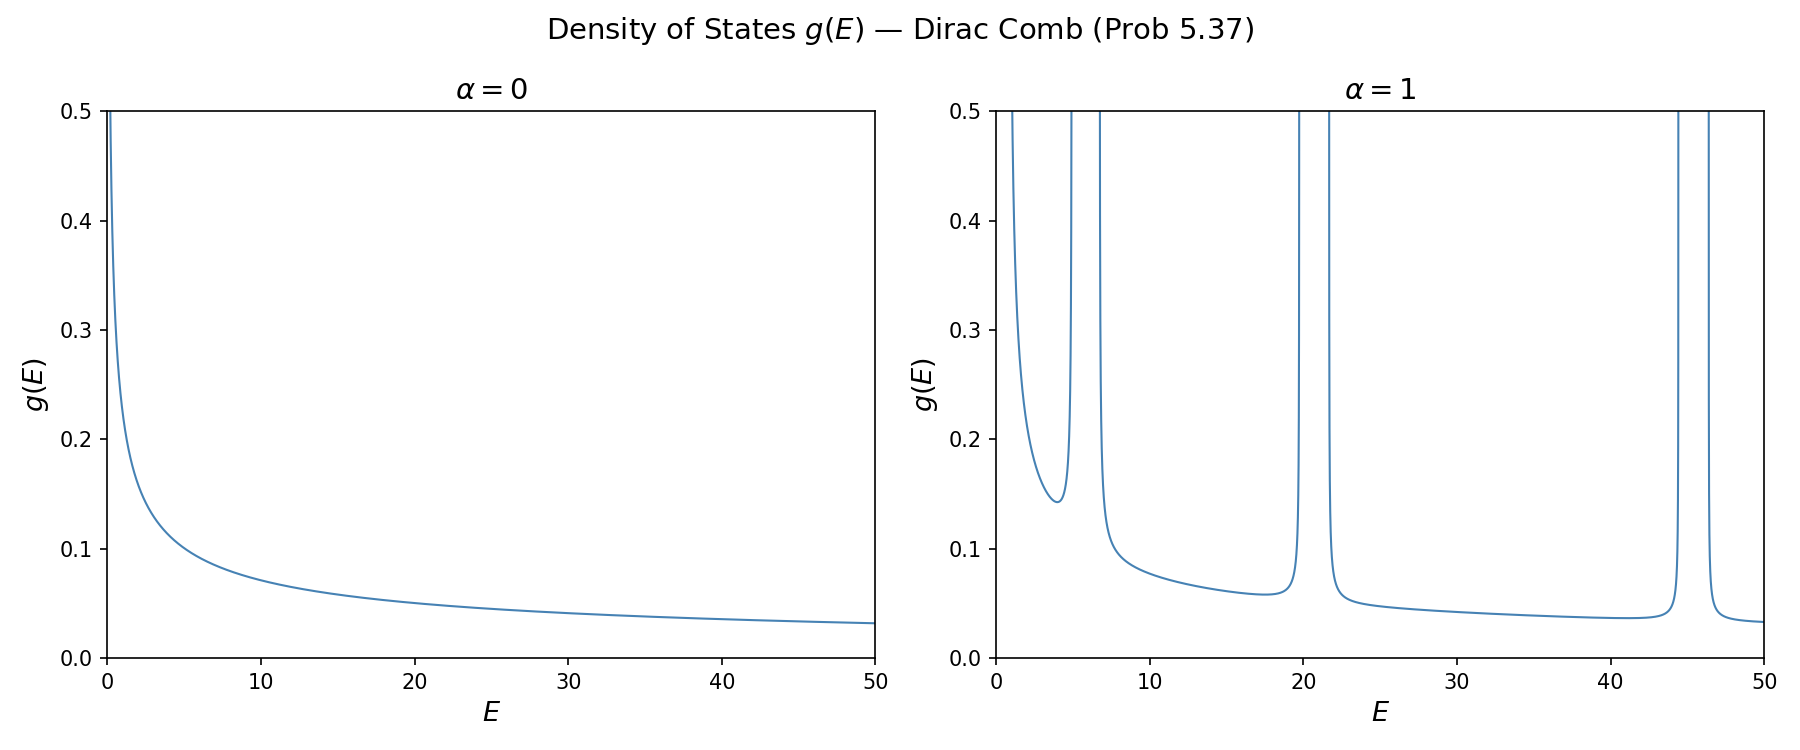
\includegraphics[width=0.8\textwidth,valign=t]{fig/prob5.37_dos.png}
   \end{enumerate}
   \subsection*{Sol. 38}
   \begin{enumerate}
       \item 
       \begin{align*}
           \frac{1}{N}
           \sum_{j=1}^N
           e^{i2\pi j(k-k')/N}
           = & 
           \frac{1}{N}
           \frac{e^{i2\pi(k-k')/N}(1-e^{i2\pi(k-k')})}{1-e^{i2\pi(k-k')/N}}
       \end{align*}
       If $k\neq k',$ the numerator is $0.$ If $k=k',$
       the sum directly says $1.$
    
        \begin{align*}
           \frac{1}{N}
           \sum_{j=1}^N
           e^{i2\pi j(k+k')/N}
           = & 
           \frac{1}{N}
           \frac{e^{i2\pi(k+k')/N}(1-e^{i2\pi(k+k')})}{1-e^{i2\pi(k+k')/N}},
       \end{align*}
       which equals $0$ except for $k+k'=N.$ If $k'=N-k,$ it equals $1.$

       \item 
       \begin{align*}
           [\hat a_{k-}, \hat a_{k'+}]
           =&\bigg[
           \frac{1}{\sqrt{N}}
           \sum_{j=1}^N e^{-i2\pi jk /N}
           \left(\sqrt{\frac{m\omega_k}{2\hbar}}x_j+
           \sqrt{\frac{\hbar}{2m\omega_k}}\frac{\partial}{\partial x_j}\right),\\
           &\frac{1}{\sqrt{N}}
           \sum_{s=1}^N e^{i2\pi sk' /N}
           \left(\sqrt{\frac{m\omega_{k'}}{2\hbar}}x_s-
           \sqrt{\frac{\hbar}{2m\omega_{k'}}}\frac{\partial}{\partial x_s}\right)
           \bigg]\\
           =&
           \frac{1}{N}
           \sum_{s,j=1}^N
           e^{-i2\pi jk /N}
           e^{i2\pi sk' /N}
           (
            -\sqrt{\frac{m\omega_k}{2\hbar}}\sqrt{\frac{\hbar}{2m\omega_{k'}}}
            [x_j, \frac{\partial}{\partial x_s}]
           +\sqrt{\frac{m\omega_{k'}}{2\hbar}}\sqrt{\frac{\hbar}{2m\omega_{k}}}
           [\frac{\partial}{\partial x_j}, x_s]
           )\\
           =&
           \frac{1}{N}
           \sum_{j=1}^N
           e^{i2\pi j(k'-k)/N}
            (
            \sqrt{\frac{\omega_k}{4\omega_{k'}}}
           +\sqrt{\frac{\omega_{k'}}{4\omega_k}}
           )\\
           =&\delta_{k,k'}.
       \end{align*}
       \begin{align*}
           [\hat a_{k-}, \hat a_{k'-}]
           =&\bigg[
           \frac{1}{\sqrt{N}}
           \sum_{j=1}^N e^{-i2\pi jk /N}
           \left(\sqrt{\frac{m\omega_k}{2\hbar}}x_j+
           \sqrt{\frac{\hbar}{2m\omega_k}}\frac{\partial}{\partial x_j}\right),\\
           &\frac{1}{\sqrt{N}}
           \sum_{s=1}^N e^{i2\pi sk' /N}
           \left(\sqrt{\frac{m\omega_{k'}}{2\hbar}}x_s+
           \sqrt{\frac{\hbar}{2m\omega_{k'}}}\frac{\partial}{\partial x_s}\right)
           \bigg]\\
           =&
           \frac{1}{N}
           \sum_{s,j=1}^N
           e^{-i2\pi jk /N}
           e^{i2\pi sk' /N}
           (
            \sqrt{\frac{m\omega_k}{2\hbar}}\sqrt{\frac{\hbar}{2m\omega_{k'}}}
            [x_j, \frac{\partial}{\partial x_s}]
           +\sqrt{\frac{m\omega_{k'}}{2\hbar}}\sqrt{\frac{\hbar}{2m\omega_{k}}}
           [\frac{\partial}{\partial x_j}, x_s]
           )\\
           =&
           \frac{1}{N}
           \sum_{j=1}^N
           e^{i2\pi j(k'-k)/N}
            (
            -\sqrt{\frac{\omega_k}{4\omega_{k'}}}
           +\sqrt{\frac{\omega_{k'}}{4\omega_k}}
           )\\
           =&0.
       \end{align*}
       \begin{align*}
           [\hat a_{k+}, \hat a_{k'+}]
           =&\bigg[
           \frac{1}{\sqrt{N}}
           \sum_{j=1}^N e^{-i2\pi jk /N}
           \left(\sqrt{\frac{m\omega_k}{2\hbar}}x_j-
           \sqrt{\frac{\hbar}{2m\omega_k}}\frac{\partial}{\partial x_j}\right),\\
           &\frac{1}{\sqrt{N}}
           \sum_{s=1}^N e^{i2\pi sk' /N}
           \left(\sqrt{\frac{m\omega_{k'}}{2\hbar}}x_s-
           \sqrt{\frac{\hbar}{2m\omega_{k'}}}\frac{\partial}{\partial x_s}\right)
           \bigg]\\
           =&
           \frac{1}{N}
           \sum_{s,j=1}^N
           e^{-i2\pi jk /N}
           e^{i2\pi sk' /N}
           (
            -\sqrt{\frac{m\omega_k}{2\hbar}}\sqrt{\frac{\hbar}{2m\omega_{k'}}}
            [x_j, \frac{\partial}{\partial x_s}]
           -\sqrt{\frac{m\omega_{k'}}{2\hbar}}\sqrt{\frac{\hbar}{2m\omega_{k}}}
           [\frac{\partial}{\partial x_j}, x_s]
           )\\
           =&
           \frac{1}{N}
           \sum_{j=1}^N
           e^{i2\pi j(k'-k)/N}
            (
            \sqrt{\frac{\omega_k}{4\omega_{k'}}}
           -\sqrt{\frac{\omega_{k'}}{4\omega_k}}
           )\\
           =&0.
       \end{align*}
    \item 
    \begin{align*}
        &\hat a_{k-}+ \hat a_{N-k+}\\
        =& 
        \frac{1}{\sqrt{N}}
        \left(
        e^{-i2\pi k/N}
        \left[
        \sqrt{\frac{m\omega_k}{2\hbar}}x_1
        +
        \sqrt{\frac{\hbar}{2m\omega_k}}\frac{\partial}{\partial x_1}
        \right]
        +\dots 
        +
        e^{-i2\pi Nk/N}
        \left[
        \sqrt{\frac{m\omega_k}{2\hbar}}x_N
        +
        \sqrt{\frac{\hbar}{2m\omega_k}}\frac{\partial}{\partial x_N}
        \right]
        \right)\\
        +&
        \frac{1}{\sqrt{N}}
        \bigg(
        e^{i2\pi (N-k)/N}
        \left[
        \sqrt{\frac{m\omega_{N-k}}{2\hbar}}x_1
        -
        \sqrt{\frac{\hbar}{2m\omega_{N-k}}}\frac{\partial}{\partial x_1}
        \right]\\
        &+\dots 
        +
        e^{i2\pi N(N-k)/N}
        \left[
        \sqrt{\frac{m\omega_{N-k}}{2\hbar}}x_N
        -
        \sqrt{\frac{\hbar}{2m\omega_{N-k}}}\frac{\partial}{\partial x_N}
        \right]
        \bigg)\\
        =&
        \frac{1}{\sqrt{N}}
        \left(
        e^{-i2\pi k/N}
        \left[
        \sqrt{\frac{m\omega_k}{2\hbar}}x_1
        +
        \sqrt{\frac{\hbar}{2m\omega_k}}\frac{\partial}{\partial x_1}
        \right]
        +\dots 
        +
        e^{-i2\pi Nk/N}
        \left[
        \sqrt{\frac{m\omega_k}{2\hbar}}x_N
        +
        \sqrt{\frac{\hbar}{2m\omega_k}}\frac{\partial}{\partial x_N}
        \right]
        \right)\\
        +&
        \frac{1}{\sqrt{N}}
        \bigg(
        e^{-i2\pi k/N}
        \left[
        \sqrt{\frac{m\omega_{k}}{2\hbar}}x_1
        -
        \sqrt{\frac{\hbar}{2m\omega_{k}}}\frac{\partial}{\partial x_1}
        \right]
        +\dots +
        e^{-i2\pi Nk/N}
        \left[
        \sqrt{\frac{m\omega_k}{2\hbar}}x_N
        -
        \sqrt{\frac{\hbar}{2m\omega_k}}\frac{\partial}{\partial x_N}
        \right]
        \bigg)\\
        =&
        \frac{2}{\sqrt{N}}
        \sqrt{\frac{m\omega_k}{2\hbar}}
        \sum_{s=1}^N
        e^{-i2\pi sk/N}
        x_s
    \end{align*}
    \begin{align*}
    R + \frac{1}{\sqrt{N}}\sum_{k=1}^{N-1}\sqrt{\frac{\hbar}{2 m\omega_k}}(\hat a_{k-}+ \hat a_{N-k+})e^{i2\pi jk/N}
    = & 
    R+ \frac{1}{\sqrt{N}}\sum_{k=1}^{N-1}\frac{1}{\sqrt{N}}
    \sum_{s=1}^Nx_s e^{i2\pi (j-s)k/N}
    \\
    = & R+ \frac{1}{N}\sum_{s=1}^Nx_s (N\delta_{j,s} - 1)\\
    =& x_j
    \end{align*}



    \begin{align*}
        &\hat a_{k-}- \hat a_{N-k+}\\
        =& 
        \frac{1}{\sqrt{N}}
        \left(
        e^{-i2\pi k/N}
        \left[
        \sqrt{\frac{m\omega_k}{2\hbar}}x_1
        +
        \sqrt{\frac{\hbar}{2m\omega_k}}\frac{\partial}{\partial x_1}
        \right]
        +\dots 
        +
        e^{-i2\pi Nk/N}
        \left[
        \sqrt{\frac{m\omega_k}{2\hbar}}x_N
        +
        \sqrt{\frac{\hbar}{2m\omega_k}}\frac{\partial}{\partial x_N}
        \right]
        \right)\\
        -&
        \frac{1}{\sqrt{N}}
        \bigg(
        e^{i2\pi (N-k)/N}
        \left[
        \sqrt{\frac{m\omega_{N-k}}{2\hbar}}x_1
        -
        \sqrt{\frac{\hbar}{2m\omega_{N-k}}}\frac{\partial}{\partial x_1}
        \right]\\
        &+\dots 
        +
        e^{i2\pi N(N-k)/N}
        \left[
        \sqrt{\frac{m\omega_{N-k}}{2\hbar}}x_N
        -
        \sqrt{\frac{\hbar}{2m\omega_{N-k}}}\frac{\partial}{\partial x_N}
        \right]
        \bigg)\\
        =&
        \frac{1}{\sqrt{N}}
        \left(
        e^{-i2\pi k/N}
        \left[
        \sqrt{\frac{m\omega_k}{2\hbar}}x_1
        +
        \sqrt{\frac{\hbar}{2m\omega_k}}\frac{\partial}{\partial x_1}
        \right]
        +\dots 
        +
        e^{-i2\pi Nk/N}
        \left[
        \sqrt{\frac{m\omega_k}{2\hbar}}x_N
        +
        \sqrt{\frac{\hbar}{2m\omega_k}}\frac{\partial}{\partial x_N}
        \right]
        \right)\\
        -&
        \frac{1}{\sqrt{N}}
        \bigg(
        e^{-i2\pi k/N}
        \left[
        \sqrt{\frac{m\omega_{k}}{2\hbar}}x_1
        -
        \sqrt{\frac{\hbar}{2m\omega_{k}}}\frac{\partial}{\partial x_1}
        \right]
        +\dots +
        e^{-i2\pi Nk/N}
        \left[
        \sqrt{\frac{m\omega_k}{2\hbar}}x_N
        -
        \sqrt{\frac{\hbar}{2m\omega_k}}\frac{\partial}{\partial x_N}
        \right]
        \bigg)\\
        =&
        \frac{2}{\sqrt{N}}
        \sqrt{\frac{\hbar}{2m\omega_k}}
        \sum_{s=1}^N
        e^{-i2\pi sk/N}
        \frac{\partial}{\partial x_s}
    \end{align*}
    The transformation goes by $R = \frac{x_1+\dots+x_N}{N},$ 
    $r_1=\frac{x_1-x_2}{N},\dots, r_{N}=\frac{x_1-x_N}{N},$ then
    $$
    x_1 = R + r_2 + r_3+\dots + r_{N-1}
    $$
    $$
    x_2 = R - r_2 + (r_3-r_2)+\dots + (r_{N-1}-r_2)
    $$
    $$
    \vdots
    $$
    $$
    x_N = R - (r_2-r_N) + (r_3-r_N)+\dots + (r_{N-1}-r_N),
    $$
    then
    $$\frac{\partial}{\partial R}=\frac{\partial }{\partial x_1}
    \frac{\partial x_1}{\partial R}+
    \dots +\frac{\partial }{\partial x_N}\frac{\partial x_N}{\partial R}
    =\frac{\partial }{\partial x_1}+
    \dots +\frac{\partial }{\partial x_N}.
    $$
    Thus
    \begin{align*}
        \frac{1}{N}\frac{\partial}{\partial R}
        +\frac{1}{\sqrt{N}}
        \sum_{k=1}^{N-1}
        \sqrt{\frac{m\omega_k}{2\hbar}}
        (\hat a_{k-}- \hat a_{N-k+}) e^{i2\pi jk/N}   
        =& 
        \frac{1}{N}\frac{\partial}{\partial R}+
        \frac{1}{N}
        \sum_{k=1}^{N-1}\sum_{s=1}^N
        e^{i2\pi(j-s)k/N}
        \frac{\partial}{\partial x_s}\\
        =&\frac{1}{N}\frac{\partial}{\partial R}+
        \frac{1}{N}
        \sum_{s=1}^N\frac{\partial}{\partial x_s}(N\delta_{j,s}-1)\\
        =&\frac{\partial}{\partial x_j}
    \end{align*}
    

    \item 
    \begin{align*}
        &\hat a_{k+}\hat a_{k-}\\
        =&
        \frac{1}{\sqrt{N}}
        \left(
        e^{i2\pi k/N}
        \left[
        \sqrt{\frac{m\omega_k}{2\hbar}}x_1
        -
        \sqrt{\frac{\hbar}{2m\omega_k}}\frac{\partial}{\partial x_1}
        \right]
        +\dots 
        +
        e^{i2\pi Nk/N}
        \left[
        \sqrt{\frac{m\omega_k}{2\hbar}}x_N
        -
        \sqrt{\frac{\hbar}{2m\omega_k}}\frac{\partial}{\partial x_N}
        \right]
        \right)\\
        &\frac{1}{\sqrt{N}}
        \left(
        e^{-i2\pi k/N}
        \left[
        \sqrt{\frac{m\omega_k}{2\hbar}}x_1
        +
        \sqrt{\frac{\hbar}{2m\omega_k}}\frac{\partial}{\partial x_1}
        \right]
        +\dots 
        +
        e^{-i2\pi Nk/N}
        \left[
        \sqrt{\frac{m\omega_k}{2\hbar}}x_N
        +
        \sqrt{\frac{\hbar}{2m\omega_k}}\frac{\partial}{\partial x_N}
        \right]
        \right)
    \end{align*}

    There are three kinds of terms:
    \begin{align*}
        e^{i2\pi jk/N}
        \sqrt{\frac{m\omega_k}{2\hbar}}x_j
        e^{-i2\pi sk/N}
        \sqrt{\frac{m\omega_k}{2\hbar}}x_s
        =\frac{m\omega_k}{2\hbar}
        e^{i2\pi (j-s)k/N}
        x_jx_s
    \end{align*}
    \begin{align*}
        &e^{i2\pi jk/N}
        \sqrt{\frac{m\omega_k}{2\hbar}}x_j
        e^{-i2\pi sk/N}
        \sqrt{\frac{\hbar}{2m\omega_k}}\frac{\partial}{\partial x_s}
        -
        e^{i2\pi sk/N}
        \sqrt{\frac{\hbar}{2m\omega_k}}
        \frac{\partial}{\partial x_s}
        e^{-i2\pi jk/N}
        \sqrt{\frac{m\omega_k}{2\hbar}}x_j
        \\
        =&
        \frac{1}{2}e^{i2\pi(j-s)k/N}x_j\frac{\partial}{\partial x_s}
        -\frac{1}{2}e^{i2\pi(s-j)k/N}x_j\frac{\partial}{\partial x_s}
        -\frac{1}{2}e^{i2\pi(s-j)k/N}\delta_{s,j}\\
        =&i\sin(2\pi(j-s)k/N)x_j\frac{\partial}{\partial x_s}
        -\frac{1}{2}\delta_{s,j}
    \end{align*}

    \begin{align*}
        -e^{i2\pi jk/N}
        \sqrt{\frac{\hbar}{2m\omega_k}}\frac{\partial}{\partial x_j}
        e^{-i2\pi sk/N}
        \sqrt{\frac{\hbar}{2m\omega_k}}\frac{\partial}{\partial x_s}
        =-\frac{\hbar}{2m\omega_k}
        e^{i2\pi (j-s)k/N}
        \frac{\partial}{\partial x_j}\frac{\partial}{\partial x_s}.
    \end{align*}
    Note that
    \begin{align*}
        \sum_{k=1}^{N-1}
        \hbar\omega_k
        \frac{m\omega_k}{2\hbar}
        e^{i2\pi (j-s)k/N}
        x_jx_s
        =&
        -\frac{m}{2}
        x_jx_s 
        \frac{4\omega^2}{4}
        \sum_{k=1}^{N-1}
        (e^{2i(\pi k /N)}
        -2+
        e^{-2i(\pi k /N)})
        e^{i2\pi (j-s)k/N}\\
        =&
        -\frac{m}{2}
        x_jx_s 
        \omega^2
        \left[
        N\delta_{j+1,s+nN} - 1
        -2N\delta_{j,s} + 2
        +N\delta_{j+nN,s+1} - 1
        \right]
    \end{align*}
    \begin{align*}
         &\sum_{k=1}^{N-1}\hbar \omega_k
        [i\sin(2\pi(j-s)k/N)x_j\frac{\partial}{\partial x_s}
        -\frac{1}{2}\delta_{s,j}]
    \end{align*}
    Since, $\omega_k = \omega_{N-k},$ $\sin(2\pi(j-s)k/N)=-\sin(2\pi(j-s)(N-k)/N),$ the first term got canceled.
    
    
    \begin{align*}
        -\sum_{k=1}^{N-1}
        \hbar\omega_k 
        \frac{\hbar}{2m\omega_k}
        e^{i2\pi (j-s)k/N}
        \frac{\partial}{\partial x_j}\frac{\partial}{\partial x_s}
        =&
        -\frac{\hbar^2}{2m}\frac{\partial^2}{\partial x_j\partial x_s}(N\delta_{j,s}-1)
    \end{align*}
    So 
    \begin{align*}
        \sum_{k=1}^{N-1}\hbar\omega_k(\hat a_{k+}\hat a_{k-} + \frac{1}{2} )
        = & \frac{1}{N}\bigg(\sum_{s,j}
        -\frac{m}{2}
        x_jx_s 
        \omega^2
        \left[
        N\delta_{j+1,s} 
        -2N\delta_{j,s} 
        +N\delta_{j,s+1} 
        \right]\\
         & -\frac{1}{2}\hbar\delta_{s,j}\sum_{k=1}^{N-1}\omega_k
        -\frac{\hbar^2}{2m}\frac{\partial^2}{\partial x_j\partial x_s}(N\delta_{j,s}-1)
        \bigg) + \frac{1}{2}\hbar\sum_{k=1}^{N-1}\omega_k
    \end{align*}

    \begin{align*}
        & \sum_{s,j}
        -\frac{m}{2}
        x_jx_s 
        \omega^2
        \left[
        N\delta_{j+1,s+nN} 
        -2N\delta_{j,s} 
        +N\delta_{j+nN,s+1} 
        \right] \\
        = & 
        - \frac{m}{2}\omega^2N 
        (-2x_1^2-2x_2^2-\dots-2x_N^2 + 2x_1x_2 + 2x_2x_3 + \dots +2 x_{N}x_{N+1})\\
        =& \frac{m}{2}\omega^2N[(x_2-x_1)^2 + (x_3-x_2)^2 + \dots + (x_{N+1}-x_{N})^2]
    \end{align*}
    \begin{align*}
        -\frac{\hbar^2}{2(Nm)}\frac{\partial^2}{\partial R^2}
        =-\frac{\hbar^2}{2Nm}\sum_{s,j}\frac{\partial^2}{\partial x_s\partial x_j}.
    \end{align*}
    Hence 
    \begin{align*}
        &-\frac{\hbar^2}{2(Nm)}\frac{\partial^2}{\partial R^2} + \sum_{k=1}^{N-1}
        \hbar \omega_k(\hat a_{k+}\hat a_{k-} + \frac{1}{2})\\
        =& 
        -\frac{\hbar^2}{2Nm}\sum_{s,j}\frac{\partial^2}{\partial x_s\partial x_j}
        +\frac{\hbar^2}{2Nm}\sum_{s,j}\frac{\partial^2}{\partial x_s\partial x_j} 
        -\frac{\hbar^2}{2m}\sum_{j}\frac{\partial^2}{\partial x_j^2}\\
         &+ \frac{m}{2}\omega^2[(x_2-x_1)^2 + (x_3-x_2)^2 + \dots + (x_{N+1}-x_{N})^2]\\
         =& \hat H.
    \end{align*}

   

       
   \end{enumerate}
   \subsection*{Sol. 39}
   \begin{enumerate}
       \item 
       $$
       e^{i(k_x(x+l_x)+k_y y + k_zz)}
       =e^{i(k_xx+k_yy+k_zz)}
       \Rightarrow k_xl_x=2n_x\pi,
       $$
       similarly 
       $$
       k_yl_y = 2n_y\pi
       $$
       $$
       k_zl_z = 2n_z\pi.
       $$
       The k space volume is 
       $$
       \frac{2\pi}{l_x}
       \frac{2\pi}{l_y}
       \frac{2\pi}{l_z} = \frac{8\pi^3}{V}
       $$
       \item 
       $$
       \frac{4}{3}\pi k_F^3 = \frac{Nd}{2}\frac{8\pi^3}{V}
       \Rightarrow k_F = 
       (3\rho\pi^2)^{1/3}
       $$
       The rest are all the same. 
       
   \end{enumerate}